%--------------------------------------------------------------------%
%
% Berkas utama templat LaTeX.
%
% author Petra Barus, Peb Ruswono Aryan
%
%--------------------------------------------------------------------%
%
% Berkas ini berisi struktur utama dokumen LaTeX yang akan dibuat.
%
%--------------------------------------------------------------------%

\documentclass[toc=listof, 12pt, a4paper, onecolumn, oneside, final]{report}

%-------------------------------------------------------------------%
%
% Konfigurasi dokumen LaTeX untuk laporan tesis IF ITB
%
% @author Petra Novandi
%
%-------------------------------------------------------------------%
%
% Berkas asli berasal dari Steven Lolong
%
%-------------------------------------------------------------------%

% Ukuran kertas
\special{papersize=210mm,297mm}

% Setting margin
\usepackage[top=3cm,bottom=2.5cm,left=4cm,right=2.5cm]{geometry}

\usepackage{mathptmx}

% Judul bahasa Indonesia
\usepackage[bahasa]{babel}

% Format citation
\usepackage[backend=bibtex,style=ieee,citestyle=numeric]{biblatex}

\usepackage[utf8]{inputenc}
\usepackage{graphicx}
\usepackage{tabularx}
\usepackage{tabto}
\usepackage{comment}
\usepackage{amsmath}
\usepackage[labelfont=bf]{caption}	% Package dengan opsi untuk mempertebal label caption
\usepackage{enumitem}				
\usepackage{tocbibind}				% Package untuk memasukkan Daftar Pustaka ke dalam Daftar Isi
\usepackage[titles]{tocloft}				% Package untuk mengatur Daftar Isi, Daftar Gambar dan Daftar Tabel
\usepackage{float}					% Package untuk membantu penetapan lokasi gambar
\usepackage{indentfirst}			% Package untuk indentasi pada paragraf pertama
\usepackage[auto]{chappg}			% Package untuk penomoran halaman Bab-Halaman
\usepackage{titling}
\usepackage{blindtext}
\usepackage{sectsty}
\usepackage{chngcntr}
\usepackage{etoolbox}
\usepackage{hyperref}       		% Package untuk link di daftar isi.
\usepackage{titlesec}       		% Package Format judul
\usepackage{parskip}

% Line satu setengah spasi
\renewcommand{\baselinestretch}{1.5}

% Setting judul
\titlespacing*{\chapter}{0pt}{-50pt}{10pt}
\chapterfont{\centering \Large}
\titleformat{\chapter}[display]
  {\Large\centering\bfseries}
  {\chaptertitlename\ \thechapter}{0pt}
    {\Large\bfseries\uppercase}

% Setting nomor pada subbsubsubbab
\setcounter{secnumdepth}{3}
\setcounter{tocdepth}{4}

\makeatletter

\makeatother

% Counter untuk figure dan table.
\counterwithin{figure}{chapter}
\counterwithin{table}{chapter}

% Counter untuk penomoran halaman lanjut
\newcounter{savepage}

% Pengaturan caption
\captionsetup{labelsep=space}

% Pengaturan spasi untuk justify
\tolerance=1
\emergencystretch=\maxdimen
\hyphenpenalty=10000
\exhyphenpenalty=10000

% Pengaturan untuk Daftar Rumus
\newcommand{\listequationsname}{Daftar Rumus}
\newlistof{myequations}{equ}{\listequationsname}
\newcommand{\myequations}[1]{%
\addcontentsline{equ}{myequations}{\protect\numberline{\theequation}#1}\par}
\setlength{\cftmyequationsnumwidth}{2.5em}

% Pengaturan untuk title Daftar Isi, Tabel, dan Gambar
\renewcommand{\cfttoctitlefont}{\hspace*{\fill}\Large\bfseries}
\renewcommand{\cftaftertoctitle}{\hspace*{\fill}}
\renewcommand{\cftlottitlefont}{\hspace*{\fill}\Large\bfseries}
\renewcommand{\cftafterlottitle}{\hspace*{\fill}}
\renewcommand{\cftloftitlefont}{\hspace*{\fill}\Large\bfseries}
\renewcommand{\cftafterloftitle}{\hspace*{\fill}} 
\renewcommand{\cftequtitlefont}{\hspace*{\fill}\Large\bfseries}
\renewcommand{\cftafterequtitle}{\hspace*{\fill}} 

\renewcommand{\cftchappresnum}{Bab }
\renewcommand{\cftchapaftersnum}{}
\renewcommand{\cftchapnumwidth}{3.7em}

\setlength{\cftbeforetoctitleskip}{-3em}
\setlength{\cftbeforeloftitleskip}{-3em}
\setlength{\cftbeforelottitleskip}{-3em}
\setlength{\cftbeforeequtitleskip}{-3em}

\makeatletter

\makeatother

\bibliography{references}

\begin{document}

    %Basic configuration
    \title{Penerapan Jarak Levenshtein untuk Metode Normalisasi dalam \textit{Voice Assistant}}
    \date{12 Februari}
    \newcommand{\yearsidang}{2019}
    \author{Rafi Dwi Rizqullah}
    \newcommand{\nim}{18214035}

    \pagenumbering{roman}
    \setcounter{page}{0}

    \clearpage
\pagestyle{empty}

\begin{center}
\smallskip

    \Large \MakeUppercase{\bfseries \thetitle}
    \vfill

    \normalsize \MakeUppercase{Laporan Tugas Akhir}
    \vfill

    \normalsize Disusun sebagai syarat kelulusan tingkat sarjana
    \vfill

    \normalsize oleh :

    \normalsize \theauthor \\
    \normalsize NIM: \nim

    \vfill
    \begin{figure}[h]
        \centering
      	
\includegraphics[width=0.25\textwidth]{resources/cover-ganesha.png}
    \end{figure}
    \vfill

    \large
    \uppercase{
        Program Studi Sistem dan Teknologi Informasi \\
        Sekolah Teknik Elektro dan Informatika \\
        Institut Teknologi Bandung \\
    }
    \yearsidang{}

\end{center}

\clearpage

    \clearpage
\pagestyle{empty}

\begin{center}
\smallskip

    \Large \bfseries \MakeUppercase{\thetitle}
    \vfill

    \Large Laporan Tugas Akhir
    \vfill

    \large Oleh

    \Large \theauthor

    \large Program Studi Sistem dan Teknologi Informasi \\
    Sekolah Teknik Elektro dan Informatika \\
    Institut Teknologi Bandung \\

    \vfill
    \normalsize \normalfont
    Telah disetujui dan disahkan sebagai Laporan Tugas Akhir di Bandung, pada tanggal 2 November 2017.

    \vfill
    \setlength{\tabcolsep}{12pt}
    \begin{tabularx}{\textwidth}{c@{\hskip 0.2\textwidth}cc@{\hskip 0.3\textwidth}}
        & Pembimbing, & \\
        & & \\
        & & \\
        & & \\
        & & \\
        & \underline{I Gusti Bagus Baskara Nugraha ST,MT,Ph.D.} & \\
        & NIP. 19760124 201012 1 001 & 
    \end{tabularx}

\end{center}
\clearpage

    \chapter*{Lembar Pernyataan}

Dengan ini saya menyatakan bahwa:

\begin{enumerate}

    \item Pengerjaan dan penulisan Laporan Tugas Akhir ini dilakukan tanpa menggunakan bantuan yang tidak dibenarkan.
    \item Segala bentuk kutipan dan acuan terhadap tulisan orang lain yang digunakan di dalam penyusunan laporan tugas akhir ini telah dituliskan dengan baik dan benar.
    \item Laporan Tugas Akhir ini belum pernah diajukan pada program pendidikan di perguruan tinggi mana pun.

\end{enumerate}

Jika terbukti melanggar hal-hal di atas, saya bersedia dikenakan sanksi sesuai dengan Peraturan Akademik dan Kemahasiswaan Institut Teknologi Bandung bagian Penegakan Norma Akademik dan Kemahasiswaan khususnya Pasal 2.1 dan Pasal 2.2.
\vspace{15mm}

Bandung, 6 Juli 2015 \\
\\
\\
\\
\\
\theauthor


    \pagestyle{plain}

    \clearpage
\chapter*{ABSTRAK}
\addcontentsline{toc}{chapter}{Abstrak}

%taruh abstrak bahasa indonesia di sini
Teknologi \textit{voice assistant} (asisten suara) mulai berkembang pesat saat ini. Penggunaannya sudah mulai merambah kepada penggunaan sehari-hari. Namun, \textit{voice assistant} masih terbatas pada penggunaan bahasa percakapan yang baku. Sementara itu, masyarakat Indonesia terbiasa mengucapkan bahasa tidak baku dalam percakapan sehari-hari. Pengerjaan Tugas Akhir ini mencakup solusi untuk mengatasi permasalahan \textit{voice assistant} dengan kata yang tidak baku atau tidak termasuk dalam kamus kata baku. Pendekatan yang digunakan sebagai solusi adalah melakukan normalisasi teks menggunakan jarak Levenshtein.

\vspace{15mm}
Kata kunci: \textit{voice assistant}, kamus, kata baku, normalisasi, jarak Levenshtein.
\clearpage
    %\clearpage
\chapter*{ABSTRACT}
\addcontentsline{toc}{chapter}{Abstract}

%put your abstract here
Voice assistant technology is growing rapidly now. Its use has begun to spread to daily use. However, voice assistants are still limited to the use of standard conversation languages. Meanwhile, Indonesian people are accustomed to saying non-formal language in everyday conversation. The execution of this Final Project includes solutions to overcome the problem of voice assistants with non-formal words or not included in the formal word dictionary. The approach used as a solution is to normalize the text using Levenshtein distance and Jaro-Winkler distance. Test result shows that normalization using Levenshtein distance outperform the normalization using LCS distance with accuracy difference of 8.34 percent.

\vspace{15mm}
Key words: voice assistant, dictionary, non-formal word, normalization, Levenshtein distance, Jaro-Winkler distance.

\clearpage
    \chapter*{Kata Pengantar}
\addcontentsline{toc}{chapter}{Kata Pengantar}

Puji Syukur penulis panjatkan kehadirat Allah SWT, karena atas kehendak dan rahmat-Nya penulis dapat menyelesaikan penulisan Laporan Tugas Akhir dengan judul “\thetitle ” untuk memenuhi syarat dari mata kuliah Tugas Akhir serta kelulusan tingkat sarjana dari program studi Sistem dan Teknologi Informasi Institut Teknologi Bandung.

Penulis mengucapkan terima kasih kepada keluarga penulis, kedua orangtua dan seorang kakak, yang selalu mendukung penulis untuk menjalani perkuliahan serta Kerja Praktik ini. Kasih sayang dari mereka telah membawa penulis sampai pada titik ini.

Penulis mengucapkan terima kasih kepada Bapak I Gusti Bagus Baskara Nugraha ST,MT,Ph.D selaku dosen STEI ITB yang telah bersedia membimbing penulis dalam pelaksanaan Tugas Akhir dan pengerjaan laporan ini. Penulis mendapatkan pelajaran yang berharga dalam mengerjakan Tugas Akhir dan menulis laporan ini yang dapat dimanfaatkan untuk kedepannya.

Penulis juga berterima kasih kepada pihak PT. Zamrud Technology yang telah bersedia membantu penulis dalam pengerjaan Tugas Akhir ini. Penulis juga dapat mempelajari ilmu baru mengenai pengerjaan Tugas Akhir penulis selama penulis berada di sana selama 8 bulan.

Penulis juga berterima kasih kepada orang-orang PT. Zamrud Technology yang telah menerima penulis untuk menjadi bagian dari mereka.

    \titleformat*{\section}{\centering\bfseries\Large\MakeUpperCase}
    
	\clearpage
    \tableofcontents
    
    \clearpage
    {%
		\let\oldnumberline\numberline%
		\renewcommand{\numberline}{\figurename~\oldnumberline}%
		\listoffigures%
	  }
	
	\clearpage
    {%
		\let\oldnumberline\numberline%
		\renewcommand{\numberline}{\tablename~\oldnumberline}%
		\listoftables%
    }

    \clearpage
    {%
		\let\oldnumberline\numberline%
        \renewcommand{\numberline}{Rumus~\oldnumberline}%
        \listofmyequations%
        \addcontentsline{toc}{chapter}{Daftar Rumus}
    }

    \clearpage
    {%
		\let\oldnumberline\numberline%
        \renewcommand{\numberline}{Algoritme~\oldnumberline}%
        \lstlistoflistings%
    }
    %\chapter*{Daftar Singkatan}

\begin{table}[H]
    \centering
	\begin{tabularx}{\textwidth}{cXc}
        \textbf{Singkatan} & \textbf{Kepanjangan dari} & \textbf{Halaman Kemunculan Pertama} \\ \hline
        SLU & \textit{Spoken Language Understanding} & \pageref{abb:slu} \\
        CNN & \textit{Convolutional Neural Network}  & \pageref{abb:cnn}
	\end{tabularx}
\end{table}
    \newpage
    \setcounter{savepage}{\arabic{page}}

    \titleformat*{\section}{\bfseries\Large}

    %----------------------------------------------------------------%
    % Konfigurasi Bab
    %----------------------------------------------------------------%    
    \renewcommand{\chaptername}{BAB}
    \renewcommand{\thechapter}{\Roman{chapter}}
    \pagenumbering{bychapter}
    \setlength{\parindent}{1cm}
    %----------------------------------------------------------------%

    %----------------------------------------------------------------%
    % Dafter Bab
    % Untuk menambahkan daftar bab, buat berkas bab misalnya `chapter-6` di direktori `chapters`, dan masukkan ke sini.
    %----------------------------------------------------------------%
    \chapter{Pendahuluan}

\section{Latar Belakang}

Suara atau audio menjadi media yang mulai kembali populer saat ini, termasuk diantaranya adalah \textit{digital audio}. Dengan adanya media digital audio, seluruh orang dapat menghibur diri sendiri sambil melakukan kegiatan sehari-hari. Menurut data \textit{survey} dari Activate pada Juni 2015, masyarakat AS menghabiskan 39 menit per hari, atau sekitar 19 persen dari waktu total per hari, pada mobile app untuk kategori audio \parencite{activate2015tech}. Dan dari sumber data yang sama pada tahun 2014, tipikal masyarakat AS berumur 13 tahun ke atas menghabiskan waktu 4 jam 5 menit per hari untuk mendengarkan audio.

Dengan melihat data tersebut, dapat dilihat bahwa bisnis audio dapat berkembang dengan konstan, khusunya dalam bidang \textit{internet radio}. Data dari eMarketer menunjukkan peningkatan pendengar bulanan \textit{internet radio} di AS yang menembus angka 50 persen dari jumlah pengguna internet sejak tahun 2012 \parencite{2013internet}. Dengan begitu, bisnis internet radio bisa menjanjikan keuntungan yang berlimpah.

Namun, terdapat keterbatasan yang dihadapi oleh \textit{internet radio}, salah satunya adalah lamanya interaksi yang diperlukan untuk mencapai suatu tujuan tertentu, seperti mencari radio yang pas atau lagu yang ingin didengarkan. Interaksi yang dilakukan seperti mengetik dan melakukan klik ke berbagai tempat. Kebanyakan manusia dapat mengucapkan kalimat lebih cepat dibandingkan dengan mengetikkannya. Kecepatan rata-rata bicara seseorang dalam percakapan biasa berada pada rentang 120 hingga 150 kata per menit \parencite{barnard2018average}. Sedangkan, kecepatan rata-rata seseorang dalam mengetik yaitu 37 kata per menit untuk wanita dan 44 kata per menit untuk pria \parencite{ratatype}.

Untuk mengatasi keterbatasan tersebut, telah ditemukan sebuah solusi yaitu menerapkan \textit{voice assistant} untuk aplikasi, seperti apa yang sudah dilakukan oleh Google dan Apple. Hadirnya voice assistant terbukti dapat membantu interaksi manusia dengan teknologi, bahkan menurut Gartner, pada tahun 2018, 30 persen interaksi dengan teknologi akan dilakukan dengan media “\textit{conversation}” (percakapan) dengan mesin pintar \parencite{escherich2015market}.

Selain itu, berbicara dengan aplikasi \textit{voice assistant} dapat menciptakan pengalaman yang lebih baik untuk pengguna. 41 persen pengguna \textit{voice assistant} merasa bahwa berbicara dengan \textit{voice assistant} terasa seperti berbicara dengan teman atau orang lain \parencite{kleinberg2018five}. Lalu, 72 persen menggunakan aplikasi \textit{voice assistant} sebagai bagian dari rutinitas harian mereka. Terakhir, \textit{speaker} yang dilengkapi \textit{voice assistant} mempermudah pengguna untuk melakukan beberapa pekerjaan sekaligus.

Namun, \textit{voice assistant} yang ada saat ini hanya berlaku untuk bahasa-bahasa baku, termasuk di Indonesia. Padahal, kebanyakan masyarakat di Indonesia berbicara dengan menggunakan bahasa Indonesia tidak baku sehari-hari.

\section{Rumusan Masalah}

Masalah yang akan diselesaikan dalam pengerjaan Tugas Akhir ini adalah "algoritma apa yang cocok untuk pembelajaran SLU selain yang sudah ada dan dapat digunakan untuk melatih bahasa percakapan sehari-hari?"

\section{Tujuan}

Tugas Akhir ini dikerjakan untuk membuktikan bahwa terdapat algoritma lain yang cocok digunakan untuk pembelajaran bahasa percakapan yang biasa digunakan sehari-hari oleh masyarakat Indonesia.

\section{Batasan Masalah}

Batasan masalah dalam pengerjaan Tugas Akhir ini hanya terletak pada pelatihan dua aspek penting SLU, yaitu pengenalan entitas (\textit{entityt recognition}) dan klasifikasi maksud kalimat (\textit{intent classification}). Selain itu, batasan masalah juga terletak pada kata-kata yang diucapkan secara lisan saja, sehingga tidak ada kata yang disingkat.

\section{Metodologi}

Metodologi yang digunakan dalam perancangan fitur \textit{voice assistant} dalam pengerjaan Tugas Akhir ini adalah sebagai berikut:

\begin{enumerate}
	\item melakukan analisis terhadap produk terkait,
	\item melakukan studi literatur algoritma-algoritma pelatihan yang telah ada sebagai pengganti,
	\item melakukan pengembangan sistem untuk mengimplementasi algoritma yang telah ditentukan, dan,
	\item melakukan evaluasi algoritma pelatihan produk terkait dengan algoritma yang lain. 
\end{enumerate}

\section{Sistematika Pembahasan}

\begin{enumerate}[label=Bab \arabic*,itemindent=*]
	\item Pendahuluan\\
	Bab ini membahas latar belakang, tujuan, batasan masalah, metodologi, dan sistematika penulisan.
	\item Kajian Pustaka\\
	Bab ini membahas teori yang digunakan untuk menyelesaikan rumusan masalah serta analisis terhadap produk terkait.
	\item Metodologi dan Rancangan\\
	Bab ini membahas metodologi pengerjaan Tugas Akhir dan rancangan algoritma yang diajukan untuk mengatasi rumusan masalah.
	\item Hasil Pengujian\\
	Bab ini membahas hasil pengujian rancangan algoritma baru yang telah dikerjakan.
	\item Kesimpulan dan Saran\\
	Bab ini berisi kesimpulan yang didapatkan dari implementasi algoritma serta saran yang dapat digunakan untuk memperbaiki fitur kedepan.
\end{enumerate}

    \chapter{Tinjauan Pustaka}

\section{Dasar Teori}

\subsection{\textit{Natural Language Understanding} (NLU)}

Pemahaman bahasa alami, atau lebih dikenal dengan \textit{natural language understanding} (NLU), merupakan salah satu bagian dari pemrosesan bahasa alami atau \textit{natural language processing} (NLP). NLU adalah ranah dalam linguistik komputasional yang didedikasikan untuk memahami bahasa alami \parencite{harris2004voice}. Menurut Gartner, NLU diartikan sebagai pemahaman komputer terhadap struktur dan makna dari bahasa manusia, sehingga pengguna dapat berinteraksi dengan komputer menggunakan bahasa yang digunakan oleh pengguna.

Dasar dari NLU berasal dari enam bentuk pengetahuan yang diketahui dan dipelajari oleh manusia pada umumnya. Bentuk-bentuk pengetahuan tersebut didefinisikan sebagai berikut: \parencite{allen1995natural}

\begin{enumerate}
	\item pengetahuan fonetik dan fonologi, menyangkut pada bagaimana suara diubah menjadi susunan kata-kata. Dalam ilmu komputer, pengetahuan ini diatasi dengan menggunakan pengenalan suara (\textit{speech recognition}),
	\item pengetahuan morfologi, menyangkut pada bagaimana sebuah kata disusun dari beberapa morfem, seperti kata “terabaikan” disusun oleh tiga morfem, yaitu “ter-”, “abai”, dan “-kan”,
	\item pengetahuan sintaktis, menyangkut pada bagaimana kata-kata dapat disusun sehingga menjadi sebuah kalimat yang benar menurut tata bahasa,
	\item pengetahuan semantik, menyangkut bagaimana makna dari kata-kata disusun untuk membentuk makna dari sebuah kalimat,
	\item pengetahuan pragmatik, menyangkut bagaimana sebuah kalimat diartikan jika digunakan dalam konteks yang berbeda, dan,
	\item pengetahuan dunia, menyangkut memahami pengetahuan umum yang dipahami juga oleh pengguna untuk menjaga percakapan berjalan dengan semestinya.
\end{enumerate}

Pengetahuan yang termasuk ke dalam NLU adalah pengetahuan sintaksis, semantik, dan pragmatik.

\subsection{\textit{Spoken Language Understanding} (SLU)}

Pemahaman bahasa ucapan, atau \textit{spoken language understanding} (SLU), merupakan ranah yang berada di antara \textit{speech recognition}, NLP yang memanfaatkan pembelajaran mesin (\textit{machine learning}) dan kecerdasan buatan (\textit{artificial intelligence}) \parencite{tur2011spoken}. Biasanya, SLU hanya terlibat dalam dua tugas utama, yaitu klasifikasi maksud kalimat (\textit{intent classification}) dan pengisian slot (\textit{slot filling}) \parencite{goo2018slot}. Karena kedua tugas utama tersebut, SLU digunakan dalam sistem yang membutuhkan satu kalimat masukan saja dan tidak terlalu panjang.

Gambar \ref{fig:slu_early} menunjukkan rancangan sistem SLU paling awal. Sistem hanya terdiri dari \textit{automatic speech recognition} (ASR) dan NLU. Tiap komponen memiliki sumber pengetahuan masing-masing, ASR memiliki ASR KS dan NLU memiliki NLU KS. Tiap sumber pengetahuan dialirkan menuju kendali pada masing-masing proses sebelum digunakan pada proses tersebut.

\begin{figure}[H]
	\centering
	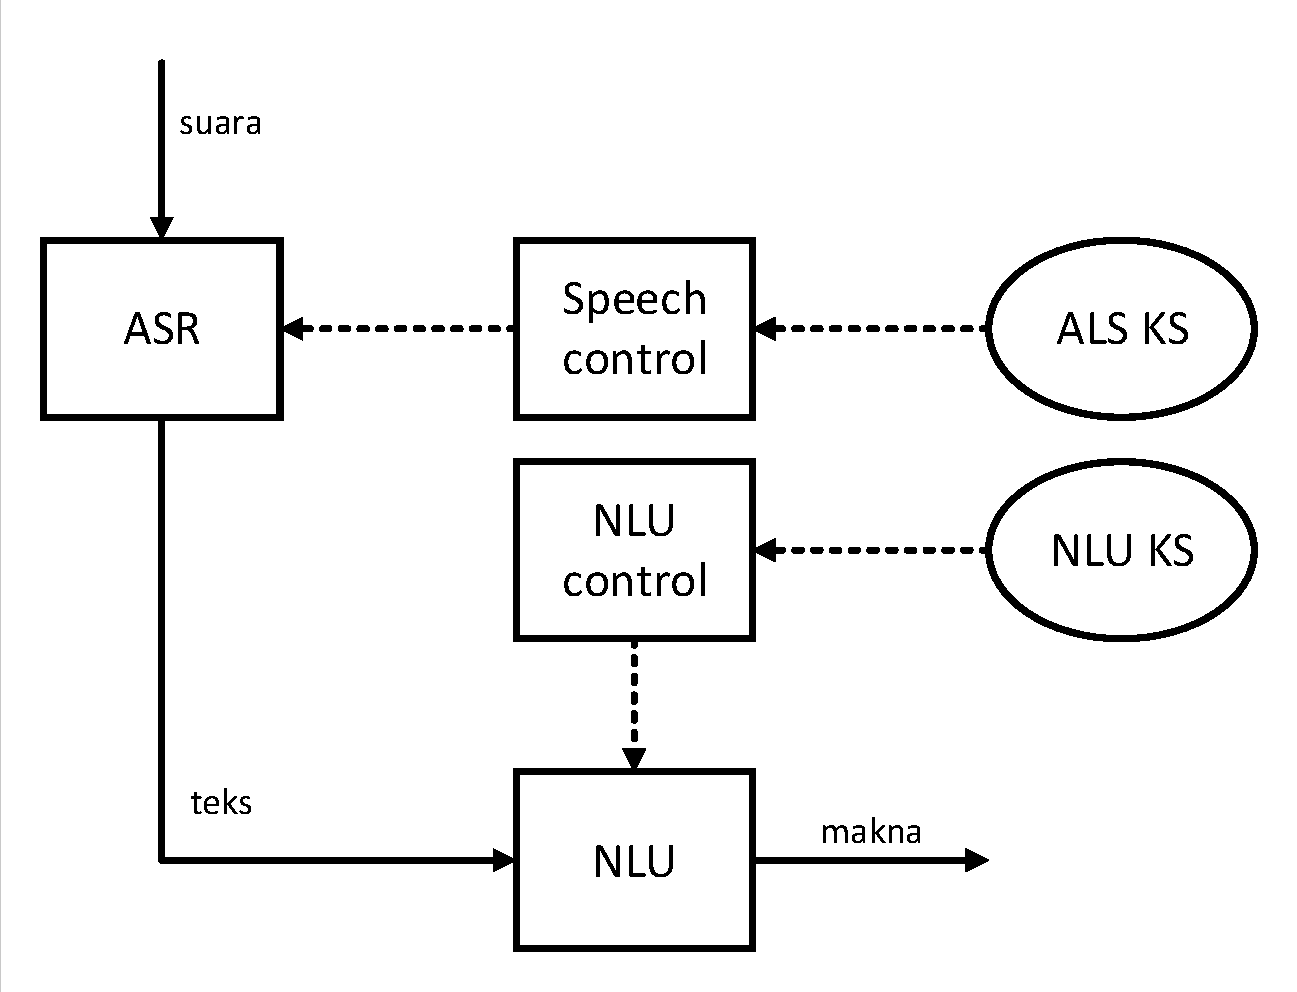
\includegraphics[width=0.5\textwidth, trim=2 2 2 2, clip]{resources/2-early_slu.pdf}
	\caption{Rancangan awal sistem SLU \parencite{tur2011spoken}}
	\label{fig:slu_early}
\end{figure}

Klasifikasi maksud kalimat berarti menentukan sebuah makna dari sebuah kalimat yang diberikan oleh pengguna. Sebagai contoh, kalimat “putarkan sebuah lagu” memiliki makna “putar media” berupa lagu. Makna tersebut kemudian diterjemahkan menjadi sebuah aksi oleh sistem. Makna kalimat bisa didapatkan dengan melihat kata-kata yang terkandung di dalam sebuah kalimat, atau melihat pola urutan kata dalam kalimat tersebut.

Pengisian slot adalah metode untuk mengambil entitas-entitas dari sebuah kalimat biasa. Beberapa aksi terkadang membutuhkan masukan parameter untuk melengkapi aksi tersebut. Masukan parameter didapatkan dari dalam kalimat yang dimasukkan oleh pengguna. Sebagai contoh, “putar lagu separuh aku dari noah” berarti pengguna menginginkan sebuah lagu diputarkan oleh sistem. Namun, permintaan pengguna menjadi lebih spesifik karena pengguna menyebutkan judul lagu beserta artis. Judul lagu adalah “separuh aku” dengan artis adalah “noah”. Metode yang dapat digunakan untuk mengambil entitas adalah melakukan pelabelan kata-kata yang menjadi entitas dengan menggunakan \textit{recurrent neural network} (RNN).

\subsection{\textit{Machine Learning}}

Pembelajaran mesin, atau \textit{machine learning}, adalah sebuah program komputer yang dirancang untuk belajar dari pengalaman dengan acuan berupa kelas tugas-tugas dan pengukuran performa, jika performa pada suatu tugas, yang telah diukur, diperbaiki dengan pengalaman \parencite{mitchell1997machine}. Pembelajaran mesin menggunakan data-data yang telah terkumpul untuk membentuk sebuah pola yang dapat digunakan pada data yang akan muncul atau dimasukkan oleh pengguna.

Pembelajaran mesin diterapkan pada berbagai macam aplikasi, yang ditujukan untuk mengurangi peran manusia dalam melakukan hal tersebut. Sebagai contoh, pembelajaran mesin digunakan untuk melakukan klasifikasi gambar, teks, suara, dan lain-lain. Selain itu, pembelajaran mesin diaplikasikan ke dalam analisis data dengan jumlah yang sangat besar atau biasa disebut sebagai \textit{big data}.

\subsection{\textit{Artificial Neural Network}}

\textit{Artificial neural network} (ANN) adalah sistem komputasi yang memiliki elemen-elemen pemrosesan sederhana yang saling terhubung, yang mana dapat memproses informasi dengan respon keadaan dinamisnya kepada masukan dari luar \parencite{caudill1987neural}. ANN terdiri dari tiga jenis lapisan, yaitu lapisan masukan, lapisan tersembunyi, serta lapisan keluaran. Lapisan masukan adalah lapisan yang berisi nilai-nilai masukan berasal dari data yang telah terkumpul. Lapisan tersembunyi berisi fungsi-fungsi aktivasi yang digunakan untuk menentukan keluaran yang diinginkan oleh \textit{neural network} secara keseluruhan.

\textit{Neural network} memiliki banyak variasi untuk kondisi data yang berbeda-beda. Jenis \textit{neural network} yang sangat dasar adalah \textit{feed forward neural network}, digunakan untuk melakukan klasifikasi sederhana. Untuk laporan ini, jenis \textit{neural network} yang digunakan adalah \textit{neural network} yang dapat digunakan dalam melakukan klasifikasi sekuensial, seperti \textit{recurrent neural network} (RNN) dan \textit{convolutional neural network} (CNN).

\section{Analisis Produk}

Produk terkait yang menjadi acuan dalam pengerjaan Tugas Akhir adalah Rasa NLU, produk NLU \textit{open source} yang dibangun oleh Rasa HQ.

\subsection{Alat-Alat yang Digunakan}

Rasa NLU merupakan salah satu bagian dari Rasa Stack, \textit{library} Python yang digunakan untuk membangun sistem \textit{chatbot} berbasis NLU. Rasa NLU membutuhkan komponen-komponen sebagai berikut: spaCy sebagai \textit{library} pembantu Rasa NLU dalam melakukan pengolahan teks, dan fastText sebagai model vektor kata yang digunakan untuk membantu spaCy dalam mengolah teks.

\subsubsection{Rasa}

Rasa, terdiri dari Rasa NLU dan Rasa Core, adalah sepasang \textit{open-source library} Python yang digunakan untuk membangun perangkat lunak berbasis percakapan \parencite{bocklisch2017rasa}. Rasa biasanya digunakan untuk pengembangan robot percakapan atau dikenal dengan \textit{chatbot} berbentuk teks. Tujuan dari Rasa adalah membantu para pengembang untuk mengembangkan manajemen dialog dan pemahaman bahasa berdasarkan pembelajaran mesin. Pengembangan Rasa terinspirasi dari beberapa \textit{library} yang telah ada, seperti scikit-learn dan Keras untuk API, fastText untuk klasifikasi teks, dan GloVe untuk penyediaan data latih untuk \textit{word embedding}. Versi Rasa yang digunakan dalam pengerjaan Tugas Akhir, yaitu Rasa NLU versi 0.11.4 dan Rasa Core versi 0.8.6.

Arsitektur Rasa dapat dilihat pada Gambar \ref{fig:rasa_arch}. Terdapat empat bagian di dalam arsitektur Rasa, yaitu \textit{Interpreter, Tracker, Policy}, dan \textit{Action}. Bagian Interpreter ditangani oleh Rasa NLU, sedangkan bagian yang lain ditangani oleh Rasa Core. Rasa bersifat modular, sehingga \textit{library} dapat diintegrasikan dengan \textit{library} lain, seperti Rasa Core dapat dihubungkan dengan \textit{Interpreter} selain Rasa NLU, dan sebaliknya.

Tahap-tahap proses yang ada di dalam arsitektur Rasa dapat dijelaskan sebagai berikut. Pertama, pesan yang dimasukkan oleh pengguna dikirimkan ke \textit{Interpreter}. Di dalam \textit{Interpreter} dilakukan proses untuk mengekstrasi \textit{intent}, entities, dan beberapa informasi terstruktur lain dari pesan yang telah dimasukkan. Kedua, luaran dari \textit{Interpreter} diteruskan menuju \textit{Tracker}. \textit{Tracker} akan melacak \textit{state} dari percakapan dan memberikan pemberitahuan baru bahwa pesan telah diterima oleh \textit{Tracker}. Ketiga, \textit{Policy} menerima  \textit{state} dari \textit{Tracker}. Keempat, \textit{Policy} menentukan \textit{Action} yang harus dilakukan sebagai tanggapan pesan dari pengguna.Kelima, \textit{Action} yang terpilih dicatat oleh \textit{Tracker}. Terakhir, \textit{Action} mulai dieksekusi kepada pengguna, baik berupa pencarian atau mengeluarkan pesan.

\begin{figure}[H]
	\centering
	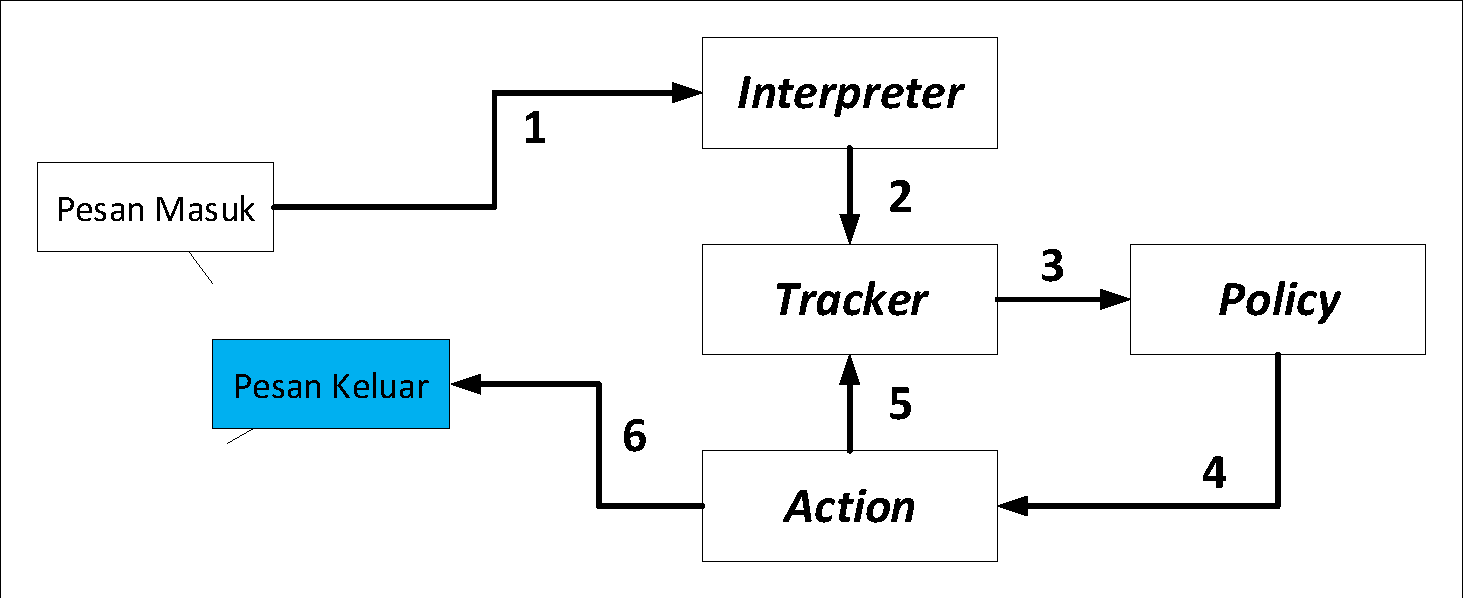
\includegraphics[width=0.9\textwidth, trim=2 2 2 2, clip]{resources/3-rasa_arch.pdf}
	\caption{Bagan arsitektur Rasa \parencite{bocklisch2017rasa}}
	\label{fig:rasa_arch}
\end{figure}

Secara sederhana, cara Rasa bekerja ditunjukkan oleh bagan pada Gambar \ref{fig:rasa_process}. Terdapat tiga proses utama dari Rasa NLU dan Rasa Core, yaitu melatih NLU, melatih dialog, dan menjalankan agen dialog.

\begin{figure}[H]
	\centering
	
\includegraphics[width=0.8\textwidth, trim=2 2 2 2, clip]{resources/3-rasa_process.pdf}
	\caption{Bagan proses utama Rasa}
	\label{fig:rasa_process}
\end{figure}

\begin{enumerate}[label=\textit{\Alph*)}, itemindent=*, series=rasa_process_list]
	\item \textit{Melatih NLU}
\end{enumerate}

Pelatihan NLU dilakukan oleh Rasa NLU dengan bantuan pengolah teks seperti spaCy dan MITIE. Pelatihan NLU berguna untuk melatih sistem untuk dapat memahami teks dan entitas didalamnya yang akan dimasukkan oleh pengguna dan menyimpan model latihan untuk digunakan saat agen dialog siap untuk dijalankan.

Untuk dapat menjalankan proses ini, dibutuhkan dua data masing-masing dalam berbentuk file JSON, yaitu data latihan dan data konfigurasi. Data latihan berisi teks masukan yang dijadikan contoh, maksud dari teks tersebut, serta entitas yang terkandung di dalamnya. Sedangkan data konfigurasi berisikan konfigurasi yang digunakan sebagai acuan dalam melatih NLU, seperti bahasa, pipeline yang digunakan untuk latihan, lokasi data latihan, dan lain-lain.

Proses-proses untuk melatih NLU dapat dilihat pada Gambar \ref{fig:rasaNLU_train}, dan penjelasan tiap proses adalah sebagai berikut:

\begin{enumerate}
	\item Rasa NLU mengambil data konfigurasi, setelah itu mengambil data latihan,
	\item memuat data latihan dan mengubahnya menjadi obyek TrainingData,
	\item memuat data konfigurasi dan mengubahnya menjadi obyek RasaNLUConfig,
	\item membuat obyek Trainer sebagai “pelatih” dan mempersiapkan obyek tersebut dengan menggunakan obyek RasaNLUConfig sebagai masukan,
	\item memanggil prosedur latihan pada obyek Trainer dengan menggunakan obyek TrainingData sebagai masukan, dan,
	\item menyimpan model hasil latihan menuju direktori sistem.
\end{enumerate}

\begin{figure}[H]
	\centering
	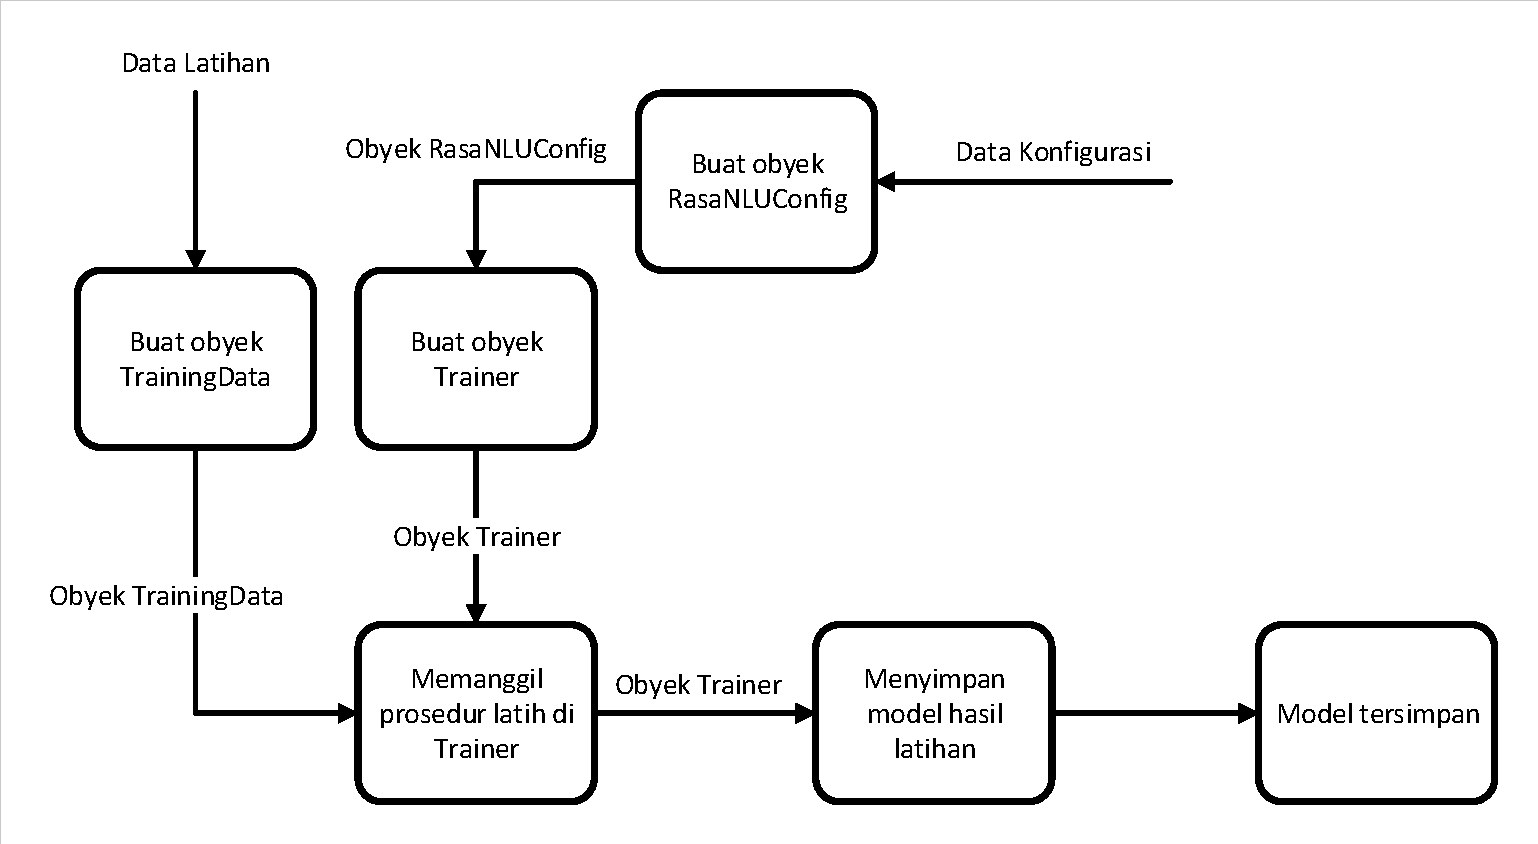
\includegraphics[width=0.8\textwidth, trim=2 2 2 2, clip]{resources/3-rasaNLU_train.pdf}
	\caption{Bagan alur latihan NLU dari Rasa NLU}
	\label{fig:rasaNLU_train}
\end{figure}

Di dalam data konfigurasi, terdapat pengaturan \textit{pipeline} yang digunakan untuk mengatur data latihan akan dilatih dengan menggunakan komponen apa saja. Alur persiapan \textit{pipeline} yang digunakan adalah, pertama menginisiasi semua komponen, lalu melakukan latihan jika terdapat prosedur latihan didalamnya, dan terakhir menyimpan hasil latihan per komponen ke dalam direktori sistem. Dalam pengerjaan Tugas Akhir ini, \textit{pipeline template} yang digunakan adalah spacy\_sklearn yang berisikan komponen latih sebagai berikut:

\begin{enumerate}
	\item nlp\_spacy, digunakan untuk inisialisasi spaCy sebelum menggunakan komponen latih spaCy yang lain,
	\item tokenizer\_spacy, digunakan untuk melakukan tokenisasi dari teks masukan dengan menggunakan tokenisasi dari spaCy,
	\item intent\_featurizer\_spacy, digunakan untuk membuat definisi ekstrasi fitur dari teks masukan dengan menggunakan spaCy. Fitur tersebut akan digunakan untuk melakukan klasifikasi maksud kalimat,
	\item intent\_entity\_featurizer\_regex, digunakan untuk mencatatkan seluruh \textit{regular expressio}n yang telah didefinisikan dalam data latihan,
	\item ner\_crf, digunakan untuk melakukan pengenalan entitas dengan menggunakan metode latihan \textit{conditional random field} (CRF) yang disediakan oleh \textit{library} sklearn-crfsuite,
	\item ner\_synonym, digunakan untuk menampung teks-teks yang memiliki nilai entitas yang sama, dan,
	\item intent\_classifier\_sklearn, digunakan untuk melakukan latihan klasifikasi maksud kalimat dengan masukan berupa fitur teks yang telah dilakukan oleh intent\_featurizer\_spacy. Latihan klasifikasi dilakukan dengan menggunakan \textit{support vector machine} (SVM) dan pengaturan parameter latih menggunakan metode \textit{grid-search} yang disediakan oleh scikit-learn.
\end{enumerate}

\begin{enumerate}[resume*=rasa_process_list]
	\item \textit{Melatih Dialog}
\end{enumerate}

Pelatihan dialog dilakukan dengan menggunakan Rasa Core. Pelatihan dialog berguna untuk mendefinisikan domain NLU dari sistem serta melatih agen dialog untuk menciptakan prediksi respon yang tepat berdasarkan masukan dari pengguna sebelumnya. Prediksi didapatkan dengan menggunakan sebuah komponen yaitu \textit{policy}.

Untuk dapat menjalankan proses ini, dibutuhkan dua data masing-masing dalam bentuk file \textit{markdown} dan YML, yaitu data cerita dan data domain. Data cerita digunakan untuk mengkonstruksi alur percakapan yang mungkin terjadi antara pengguna dengan sistem. Data cerita terdiri dari balok-balok cerita, berisi maksud kalimat yang diekstraksi dari teks masukan pengguna dan respon sistem terhadap masukan tersebut. Jumlah respon dan timbal balik dalam satu balok cerita tidak terbatas. Data domain digunakan untuk inisialisasi definisi dari maksud kalimat, entitas yang terlibat, slot yang tersedia, serta aksi yang akan dilakukan oleh sistem.

Proses-proses untuk melatih agen dialog dijelaskan sebagai berikut:

\begin{enumerate}
	\item Rasa Core mengambil data domain dan data cerita,
	\item membuat agen dialog dengan membuat obyek Agent menggunakan masukan data domain dan policy yang digunakan,
	\item memanggil prosedur latih dari obyek Agent dengan menyertakan data cerita sebagai masukan. Prosedur ini juga membuat obyek PolicyTrainer dan melakukan pelatihan, dan,
	\item menyimpan agen dialog terlatih ke dalam direktori sistem.
\end{enumerate}

\begin{enumerate}[resume*=rasa_process_list]
	\item \textit{Menjalankan Agen Dialog}
\end{enumerate}

Setelah model NLU dan agen dialog telah tersimpan ke dalam direktori, sistem sudah siap untuk menjalankan agen dialognya. Sistem akan melakukan \textit{loop} selamanya terhadap proses memasukkan teks. Teks yang telah dimasukkan oleh pengguna akan diprediksi maksud kalimatnya sehingga sistem dapat menentukan aksi yang tepat.

\subsubsection{spaCy}

spaCy adalah sebuah \textit{open-source library} Python digunakan untuk melakukan pengolahan teks, khususnya NLP, dalam tingkat industri \parencite{spacy2}. spaCy mendukung banyak bahasa selain MITIE, dan lebih mudah untuk menambahkan bahasa baru, cukup dengan menyediakan model bahasa yang dibutuhkan ke dalam spaCy. Versi spaCy yang digunakan adalah versi 2.0.11.

Arsitektur spaCy dapat terlihat di dalam Gambar \ref{fig:spaCy_arch} \parencite{spacy2}. Terdapat dua struktur data pusat yang berada di dalam spaCy, yaitu Doc dan Vocab. Doc berisi rangkaian dari \textit{token} dan semua anotasinya, sedangkan Vocab berisi sekumpulan tabel \textit{look-up} untuk menyediakan informasi umum ke seluruh dokumen, bertujuan untuk mencegah terjadinya duplikasi data dan memastikan bahwa fakta hanya tersimpan di dalam satu sumber.

Dengan menyimpan semua fakta di dalam satu sumber dapat menghemat penyimpanan di dalam arsitektur spaCy itu sendiri. Seperti, Doc menyimpan seluruh data-data anotasi teks, sedangkan Token dan Span hanya berupa \textit{view} yang berisi \textit{pointer} untuk merujuk kepada data yang ada di Doc.

\begin{figure}[H]
	\centering
	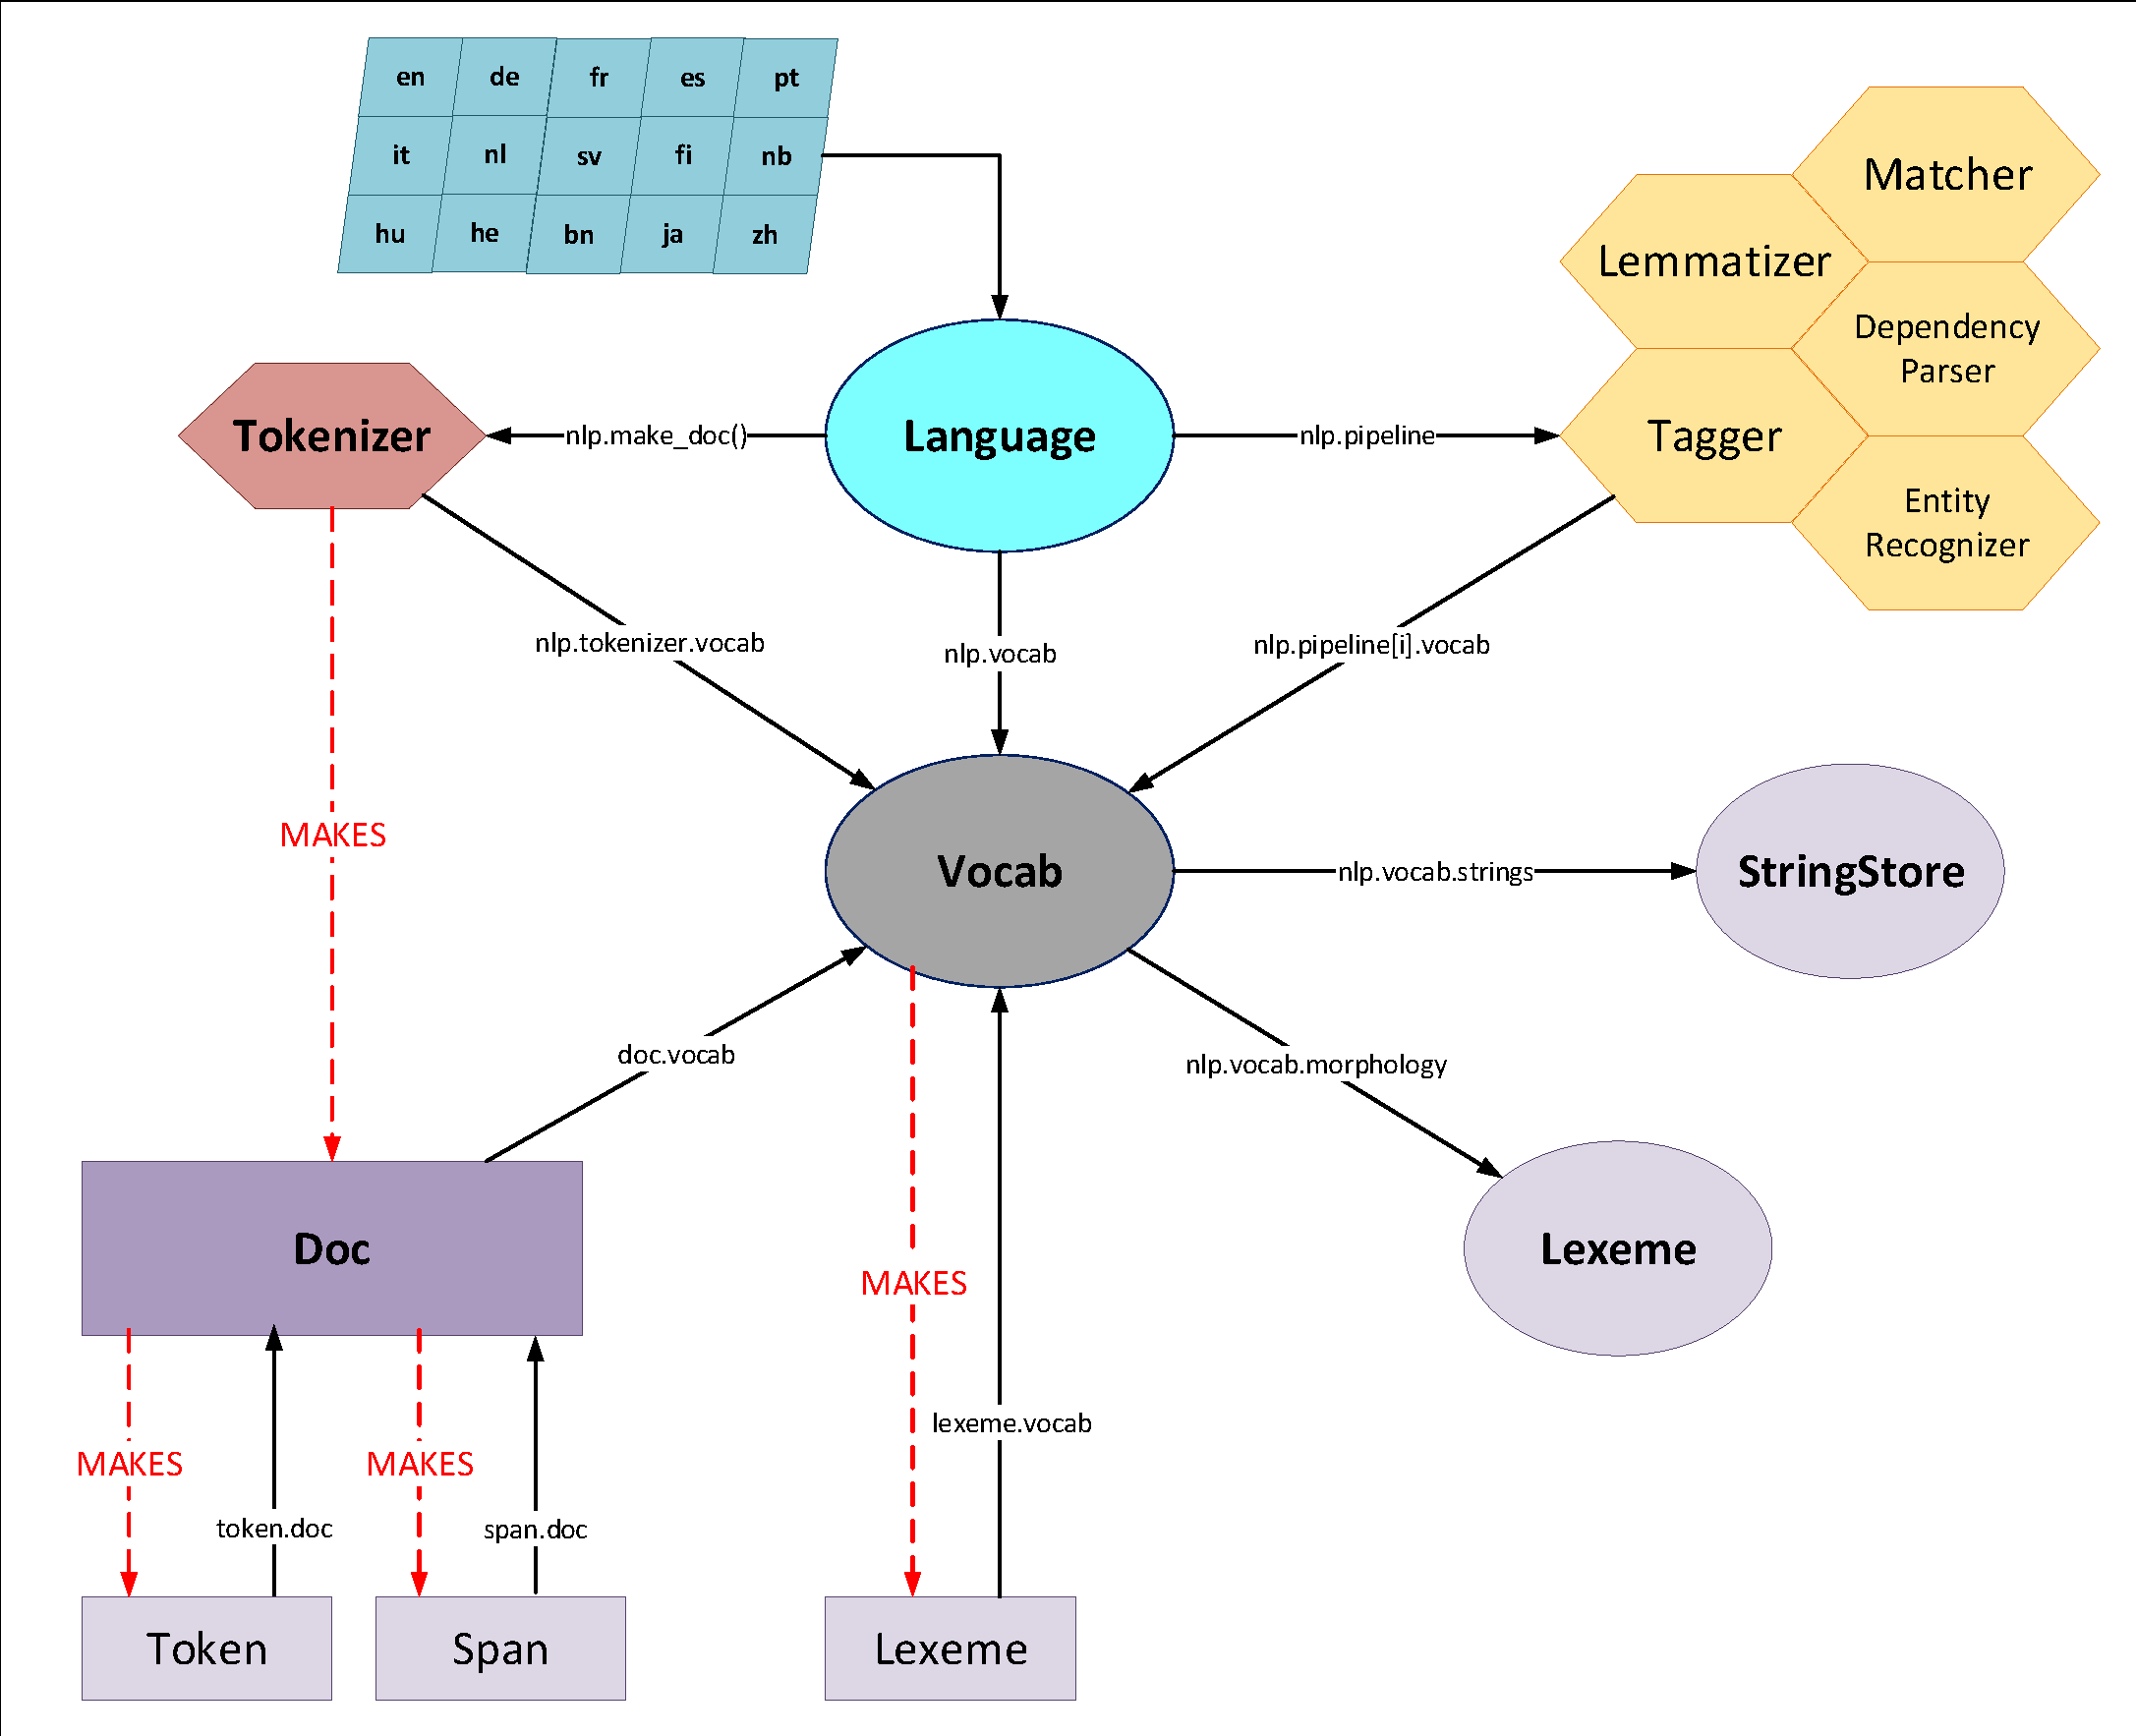
\includegraphics[width=0.9\textwidth, trim=2 2 2 2, clip]{resources/3-spacy_arch.pdf}
	\caption{Bagan arsitektur spaCy \parencite{spacy2}}
	\label{fig:spaCy_arch}
\end{figure}

\subsubsection{fastText}

fastText adalah \textit{library} untuk klasifikasi dan representasi teks yang dibangun oleh peneliti AI dari Facebook \parencite{joulin2017bag}. Pemrosesan yang dilakukan adalah mengubah sebuah kalimat-kalimat yang tersedia menjadi sebuah model vektor. Model vektor merepresentasikan kedekatan antara suatu kata dengan kata yang lain, memiliki nilai rentang antara 0 hingga 1. Model vektor tersebut dapat dipakai tidak hanya oleh \textit{library} fastText, namun juga dapat digunakan oleh \textit{library} luar, seperti spaCy.

Untuk pengerjaan Tugas Akhir ini, digunakan model vektor yang telah tersedia oleh fastText di dalam repositori GitHub. Model vektor yang digunakan adalah model vektor berbahasa Indonesia, yang diproses dari teks-teks yang tersedia di Wikipedia. Untuk dapat menggunakan model vektor, terlebih dahulu model vektor dikonversi menjadi model bahasa spaCy, dalam hal ini model bahasa Indonesia.

\subsection{Teori yang Diterapkan}

\subsubsection{Pengenalan Entitas dengan \textit{Conditional Random Field}}

\textit{Conditional random field} (CRF) adalah metode pembelajaran yang digunakan untuk data-data yang bersifat berurutan. CRF menggunakan fitur-fitur yang dimiliki oleh sebuah kata untuk melakukan pelatihan. Fitur yang digunakan untuk CRF dapat bervariasi sesuai kebutuhan, namun fitur dasar yang tersedia adalah kata utama dan kata sebelum kata utama. CRF biasanya digunakan untuk \textit{sequence labelling} teks.

Rasa NLU menggunakan \textit{library} Python yaitu sklearn-crfsuite. \textit{Library} ini merupakan pembungkus \textit{library} python-crfsuite yang mana menyediakan \textit{estimator} yang cocok dengan scikit-learn \parencite{sklearncrf}. Hal tersebut memudahkan penggunaan model CRF untuk pelatihan dan menyimpan model hasil latihan. Selain itu, spaCy juga menyediakan fitur yang dapat digunakan oleh CRF milik Rasa NLU, yaitu fitur POS \textit{tag} untuk tiap kata dalam kalimat.

\subsubsection{Klasifikasi Maksud Kalimat dengan \textit{Support Vector Machine}}

\textit{Support vector machine} (SVM), atau \textit{support vector network}, adalah sebuah metode pembelajaran yang memetakan vektor masukan menjadi ruang fitur dengan dimensi yang tinggi melalui pemetaan non linear yang telah dipilih sebelumnya \parencite{cortes1995support}. SVM biasanya digunakan untuk menjelaskan kegiatan klasifikasi dengan metode support vector, namun kegunaan SVM juga bisa digunakan untuk kegiatan regresi. Oleh karena itu, SVM terbagi menjadi dua, yaitu \textit{support vector classification} (SVC) untuk klasifikasi dan \textit{support vector regression} (SVR) untuk regresi \parencite{gunn1998support}.

Rasa NLU menggunakan SVM untuk melakukan klasifikasi maksud kalimat dari scikit-learn. Dengan jumlah maksud kalimat yang berjumlah lebih dari dua, maka scikit-learn akan menggunakan metode-metode untuk mengakali SVM sehingga dapat digunakan untuk kasus melakukan klasifikasi lebih dari dua kelas. Selain itu, Rasa menggunakan metode \textit{grid-search} untuk melakukan \textit{hyperparameter tuning.}

\subsection{Analisis Kekurangan Sistem}

Selama pengerjaan sistem NLU berlangsung, terdapat kekurangan-kekurangan yang dimiliki oleh alat-alat yang digunakan untuk membangun sistem. Kekurangan tersebut berkaitan dengan permasalahan proyek yang sedang dikerjakan.

%\subsubsection{Model yang Digunakan Tidak Cukup}
%
%Model vektor fastText digunakan untuk dapat membangun model bahasa Indonesia spaCy, dan digunakan dalam melakukan pengolahan teks di Rasa. Namun, model bahasa yang berhasil dibangun dari model vektor hanyalah pada bagian kosakata saja. Untuk dapat membangun model bahasa yang baik, model juga memerlukan bagian-bagian seperti \textit{named entity recognition}, \textit{parser}, serta \textit{tagger}.
%
%\textit{Named entity recognition}, atau NER, merujuk kepada pengenalan \textit{token-token} yang merupakan sebuah entitas, seperti nama oganisasi, nama tempat, tanggal, waktu, angka urutan, dan lain-lain. NER diperlukan untuk membedakan antara \textit{token} biasa dengan \textit{token} entitas. \textit{Parser} merujuk kepada \textit{dependency parsing} yaitu melihat ketergantungan sebuah token dengan token yang lain. Sebagai contoh, kalimat “Budi memakan nasi” memiliki dua ketergantungan, yaitu “Budi” memiliki ketergantungan subyek dengan “memakan”, dan “nasi” memiliki ketergantungan obyek dengan “memakan”. Terakhir, \textit{tagger} merujuk kepada \textit{POS tagging} yaitu memberikan tanda kepada token berdasarkan sifat kata dari token tersebut, misal kata kerja, kata benda, tanda baca, dan lain-lain.
%
%Terdapat beberapa korpus untuk latihan yang menyediakan komponen seperti \textit{dependency parser} dan \textit{POS tag}, salah satunya berasal dari Universal Dependencies. Universal Dependencies menyediakan korpus yang diambil dari berbagai sumber, seperti berita, artikel blog, istilah hukum, istilah medis, Wikipedia, dan lain-lain.
%
\subsubsection{Kebutuhan Ekstraksi Fitur untuk CRF}

CRF membutuhkan fitur-fitur yang telah didefinisikan sebelumnya untuk dapat melakukan latihan, seperti CRF yang diterapkan oleh Rasa membutuhkan fitur POS \textit{tag} pada sebuah kata. Fitur tersebut hanya bisa didapatkan dengan \textit{library} NLP, seperti spaCy, yang dapat melakukan latihan POS \textit{tag} berdasarkan model yang telah disediakan oleh pengguna. Oleh karena itu, sebuah kalimat masukan perlu melakukan klasifikasi dengan spaCy terlebih dahulu sebelum akhirnya diekstraksi dengan menggunakan Rasa.

Model vektor fastText digunakan untuk dapat membangun model bahasa Indonesia spaCy, dan digunakan dalam melakukan pengolahan teks di Rasa. Namun, model bahasa yang berhasil dibangun dari model vektor hanyalah pada bagian kosakata saja. Untuk dapat membangun model bahasa yang baik, model juga memerlukan bagian-bagian seperti POS \textit{tagger}. Kekurangan informasi tersebut berakibat pada klasifikasi spaCy yang menjadi tidak maksimal.

Lalu, model dari fastText hanya tersedia dalam bahasa Indonesia yang baku. Hal ini dapat menyebabkan kesulitan dalam mengenal kata-kata yang baru diucapkan, atau kata yang tidak baku seperti kata-kata dalam percakapan sehari-hari. Oleh karena itu, pendekatan CRF dari Rasa NLU tidak cocok untuk digunakan pada proyek ini.

\subsubsection{Penggunaan SVM untuk Klasifikasi Lebih dari Dua Kelas}

Rasa NLU menggunakan metode SVM dengan tambahan pengaturan grid-search dari scikit-learn untuk melakukan pelatihan klasifikasi maksud kalimat. Kelemahan yang terdapat pada SVM dalam melakukan klasifikasi adalah SVM hanya dapat melakukan klasifikasi pada dua kelas saja. SVM tidak dirancang untuk mengatasi permasalahan klasifikasi yang membutuhkan lebih dari dua kelas. Namun, scikit-learn dapat mengatasi permasalahan tersebut dengan menggunakan skema klasifikasi one-versus-one. Skema tersebut bekerja dengan cara membuat satu alat klasifikasi untuk tiap pasangan kelas yang ada. Pada saat prediksi, kelas yang menerima voting tertinggi akan terpilih [cit].

Kelemahan yang dimiliki oleh skema one-versus-one adalah jumlah klasifikasi yang dilakukan, yaitu (jumlah kelas * (jumlah kelas – 1) / 2) klasifikasi, membuat skema ini memiliki kompleksitas O(jumlah kelas \^{} 2). Dengan jumlah klasifikasi yang banyak, SVM dirasa tidak efisien untuk melakukan klasifikasi dengan jumlah kelas yang banyak. Oleh karena itu, metode klasifikasi yang tepat digunakan untuk mengatasi masalah jumlah kelas lebih dari dua tersebut adalah \textit{neural network}.

Keluaran dari \textit{neural network} dapat diatur sesuai dengan jumlah kelas yang tersedia pada data latihan. Fleksibilitas yang dimiliki oleh \textit{neural network} membuat metode ini dapat melakukan satu model dan satu kali latihan klasifikasi untuk dapat menghasilkan model yang bagus untuk digunakan.
    \chapter{Normalisasi Teks dengan Jarak Levenshtein}

\section{Alur Proses Normalisasi Teks dengan Jarak Levenshtein}

Gambar \ref{fig:side_to_side} bagian (a) menunjukkan alur proses untuk rancangan metode normalisasi yang diusulkan. Metode normalisasi usulan menggunakan jarak Levenshtein sebagai penghitungan jarak antara kedua teks. Deskripsi alur proses yang dijalankan dapat dijelaskan sebagai berikut:
\begin{enumerate}
	\item diberikan kata masukan dan kamus kata baku,
	\item melakukan pencarian kata-kata dalam kamus kata baku yang memiliki jarak minimum dengan kata masukan menggunakan jarak Levenshtein, menghasilkan kumpulan kata, dan,
	\item melakukan seleksi kata yang menjadi kata keluaran. Jika terdapat lebih dari satu kata, maka kata yang dipilih adalah kata yang pertama kali ditemukan.
\end{enumerate}
\begin{figure}[ht]
	\centering
	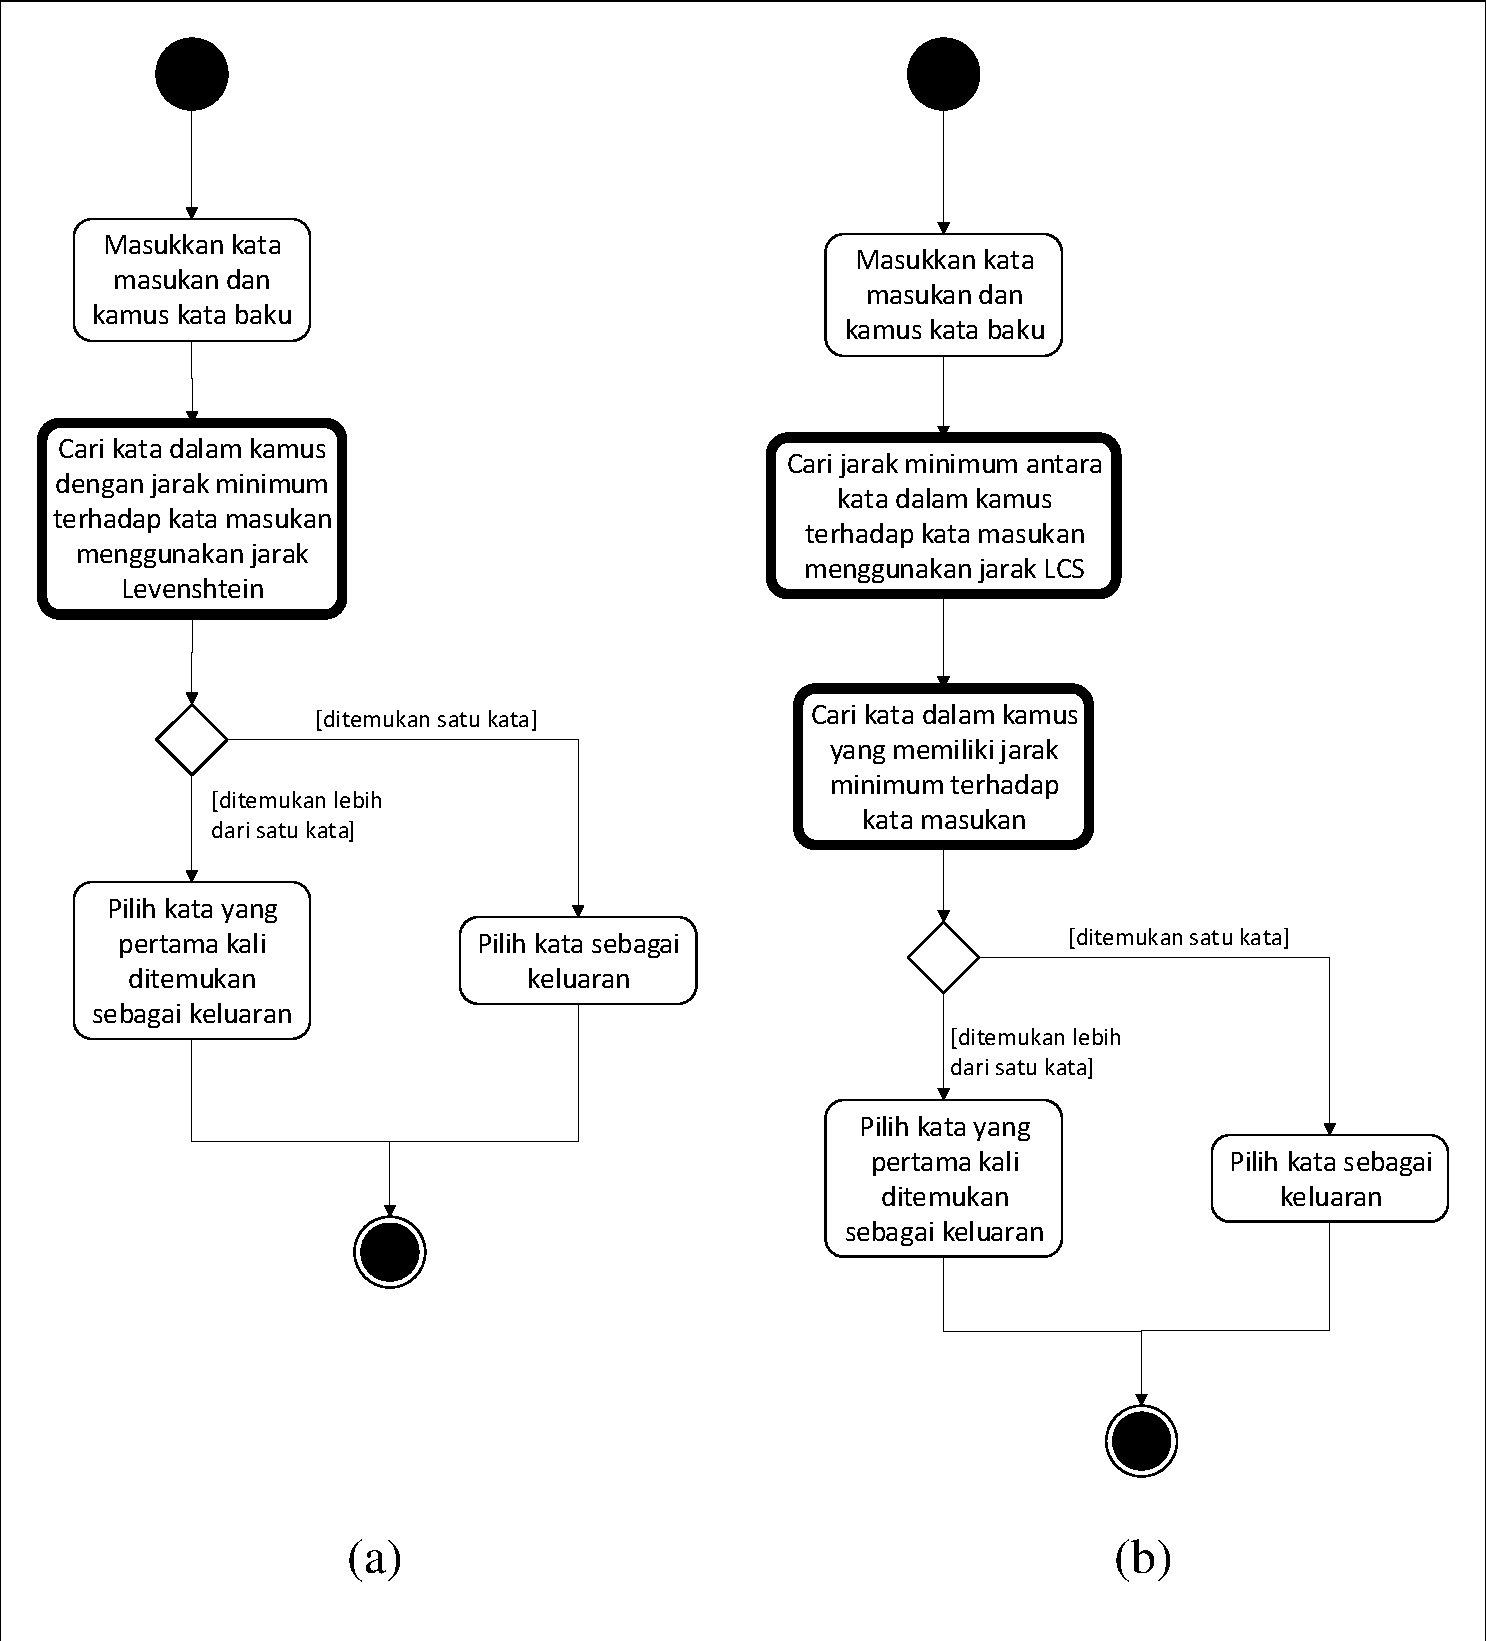
\includegraphics[width=0.8\textwidth, trim=2 2 2 2, clip]{resources/3/side_to_side.pdf}
	\caption{Alur proses normalisasi teks dengan (a) jarak Levenshtein, dan (b) jarak LCS \parencite{saragih2017normalisasi}}
	\label{fig:side_to_side}
\end{figure}

Terdapat perbedaan alur proses antara metode normalisasi \parencite{saragih2017normalisasi} dengan metode normalisasi menggunakan jarak Levenshtein. Perbedaan tersebut dapat dilihat pada blok proses dengan garis tepi tebal pada Gambar \ref{fig:side_to_side}. Perbedaan pertama terletak pada penggantian algoritme jarak LCS dengan jarak Levenshtein. Kedua, metode normalisasi usulan mempersingkat proses normalisasi dengan menemukan kumpulan kata prediksi dengan jarak minimum secara langsung dibandingkan metode normalisasi \parencite{saragih2017normalisasi} yang harus mencari jarak minimum terlebih dahulu kemudian menemukan kumpulan kata prediksi dengan jarak tersebut.

\section{Algoritme Normalisasi Teks dengan Jarak Levenshtein}

Algoritme \ref{lst:lv} merupakan algoritme persamaan jarak Levenshtein yang dapat dilihat pada Rumus \ref{eq:lv} \parencite{levenshtein1966binary}. Algoritme menerima masukan berupa dua kata dan mengeluarkan nilai jarak perubahan berupa bilangan bulat. Penghitungan jarak perubahan kedua kata masukan dilakukan dengan menggunakan matriks dua dimensi dengan ukuran matriks disesuaikan dengan kedua masukan kata tersebut.
\begin{lstlisting}[caption={Algoritme Fungsi Jarak Levenshtein},label={lst:lv},float,floatplacement=H]
Masukan: str1, str2		: string
Keluaran: integer

Deklarasi:
str1, str2 				: string
len1, len2, i, j, actv 	: integer
matrix					: array[][] integer

Deskripsi:
Mulai
1. Menambah str1 dan str2 dengan spasi di depan;
2. masukkan secara berurutan nilai panjang str1 dan str2 ke dalam variabel len1 dan len2;
3. membuat matrix dengan ukuran len1 x len2 lalu isi semua sel dengan nilai 0;
4. selama i diantara 1 dan len1 - 1, isi sel matrix[i][0] dengan nilai i;
5. selama j diantara 1 dan len2 - 1, isi sel matrix[0][j] dengan nilai j;
6. selama i diantara 1 dan len1 - 1 dan j diantara 1 dan len2 - 1:
	a) masukkan variabel actv dengan nilai 1;
	b) jika str1[i] sama dengan str2[j], ubah nilai actv dengan nilai 0;
	c) masukkan variabel matrix[i][j] dengan nilai terkecil antara matrix[i-1][j] + 1, matrix[i][j-1] + 1, atau matrix[i-1][j-1] + actv.
7. keluarkan nilai dalam variabel matrix[len1-1][len2-1].
Selesai
\end{lstlisting}

Fungsi dalam Algoritme \ref{lst:lv} digunakan untuk metode normalisasi kata pada Algoritme \ref{lst:lev_find} dengan tujuan untuk mencari kumpulan kata yang memiliki jarak perubahan paling kecil. Terdapat dua masukan metode yaitu sebuah kata dan sebuah kamus dalam bentuk vektor. Metode menghasilkan dua keluaran, yaitu nilai jarak terkecil antara kata masukan dengan seluruh kata dalam kamus dan vektor berisi kumpulan kata dengan jarak terkecil dengan kata masukan.
\begin{lstlisting}[caption={Algoritme Fungsi Normalisasi Kata dengan Jarak Levenshtein},label={lst:lev_find},float,floatplacement=h]
Masukan: txt : string, kam : dictionary
Keluaran: array, integer

Deklarasi:
txt, word		: string
val, minVal 	: integer
kam				: dictionary
similarWords	: array[] string

Deskripsi:
Mulai
1. Masukkan nilai 30 ke dalam variabel minVal;
2. masukkan nilai txt ke dalam vektor similarWords;
3. untuk seluruh kata dalam kam:
	a) Masukkan nilai kata ke dalam variabel word;
	b) hitung jarak Levenshtein antara txt dengan word, simpan hasil ke dalam variabel val;
	c) jika val lebih kecil dari minVal:
		i) jika val sama dengan nol (0), jadikan word sebagai vektor lalu keluarkan vektor bersama dengan nilai 0;
		ii) jika val tidak sama dengan nol, ganti similarWords dengan vektor berisi word lalu ganti minVal dengan val.
	d) jika val sama dengan minVal, tambah nilai ke dalam array similarWords.
4. keluarkan array similarWords dan nilai dalam variabel minVal.
Selesai
\end{lstlisting}

Berbagai kondisional yang tercantum dalam Algoritme \ref{lst:lev_find} dijelaskan sebagai berikut:
\begin{enumerate}
	\item "jika \textit{val} sama dengan nol (0)" yaitu kata masukan (\textit{txt}) dan kata dalam kamus (\textit{word}) adalah kata yang sama persis, ditunjukkan dengan jarak perubahan (\textit{val}) bernilai nol. Oleh karena itu, \textit{word} langsung diubah menjadi vektor lalu dijadikan sebagai keluaran fungsi beserta nilai jaraknya yaitu nol;
	\item "jika \textit{val} tidak sama dengan nol" yaitu ditemukan \textit{word} dengan jarak yang lebih kecil dibandingkan jarak terkecil (\textit{minVal}) sebelumnya sehingga seluruh isi vektor kumpulan kata (\textit{similarWords}) terdahulu harus dibuang lalu digantikan dengan \textit{word}; dan
	\item "jika \textit{val} sama dengan \textit{minVal}" yaitu ditemukan \textit{word} yang memiliki jarak yang sama dengan seluruh kata dalam \textit{similarWords} sehingga \textit{word} harus dimasukkan ke dalam \textit{similarWords}.
\end{enumerate}

\section{Contoh Normalisasi Teks dengan Jarak Levenshtein}

Contoh normalisasi teks dengan jarak Levenshtein tertera pada Tabel \ref{tbl:eg_output}. Salah satu contoh yang digunakan adalah kata "\textit{mikir}". Kata "\textit{mikir}" memiliki keluaran kumpulan kata-kata baku, yaitu "pikir", "bikir", "kikir", "likir", "milir", dan "zikir". Semua kata baku tersebut memiliki jarak perubahan yang sama dengan kata "\textit{mikir}" yaitu 1. Jarak tersebut juga merupakan jarak terkecil yang dapat dicapai antara kata masukan dengan seluruh kata yang ada di dalam kamus.
\begin{table}[ht]
    \captionsetup{justification=justified,singlelinecheck=false}
    \caption{Contoh keluaran Normalisasi Teks dengan Jarak Levenshtein}
    \label{tbl:eg_output}
    \centering
    \begin{tabularx}{\textwidth}{|Y|X|X|}
        \hline
        \textbf{Contoh kata masukan} & \multicolumn{1}{Y|}{\textbf{Contoh keluaran kumpulan kata}} & \multicolumn{1}{Y|}{\textbf{Contoh keluaran jarak terkecil}} \\ \hline
        \textit{mikir} & {[}'pikir', 'bikir', 'kikir', 'likir', 'milir', 'zikir'] & 1 \\ \hline
        \textit{maen} & {[}'main', 'man', 'men'] & 1 \\ \hline
        \textit{begimana} & {[}'bagaimana', 'begana']& 2 \\ \hline
    \end{tabularx}
\end{table}
    \chapter{Pengujian}

Bab ini membahas pengujian normalisasi teks pada metode normalisasi teks \parencite{saragih2017normalisasi}, metode normalisasi teks dengan jarak Jaro-Winkler, dan metode normalisasi teks dengan jarak Levenshtein. Pembahasan yang tertera meliputi perangkat dan lingkungan yang digunakan untuk pengujian, metode pengujian, skenario pengujian, serta hasil dan analisis pengujian.

\section{Perangkat dan Lingkungan Pengujian}

Pengujian ketiga metode dilakukan dengan menggunakan perangkat laptop dengan spesifikasi sebagai berikut:
\begin{enumerate}
    \item Spesifikasi Perangkat Keras:
    \begin{enumerate}
        \NumTabs{6}
        \setlength{\itemsep}{1pt}
        \item Perangkat \tab \tab : ASUS X450LD tahun 2014
        \item Prosessor \tab \tab : 1,6 GHz Intel Core i5 4200U
        \item Memori \tab \tab : 4 GB DDR3
        \item Penyimpanan \tab : HDD 500 GB
        \item Sistem Operasi \tab : Windows 10 64bit
    \end{enumerate}
    \item Alat Bantu Pengembangan: Visual Studio Code, Anaconda, Jupyter Notebook
    \item Bahasa Pemrograman: Python 3.6.5 64bit
    \item \textit{Library} Python yang Digunakan: \textit{csv} \parencite{pythoncsv}, \textit{textdistance} \parencite{orsiniumtext}
\end{enumerate}

\section{Metode Pengujian}

Pengujian dilakukan dengan melakukan perbandingan antara metode normalisasi teks \parencite{saragih2017normalisasi}, metode normalisasi dengan jarak Jaro-Winkler, dan metode normalisasi teks dengan jarak Levenshtein. Ketiga metode normalisasi diberikan masukan yang sama. Keluaran dari ketiga metode dinilai dengan menggunakan persentase akurasi yang disesuaikan dengan skenario yang berbeda. Penilaian persentase akurasi dilakukan dengan menggunakan persamaan:
\begin{equation*}
	\text{Persentase akurasi}=\frac{\text{x}}{y} \times 100\%
\end{equation*}
%\myequations{Penghitungan akurasi fungsi \textit{stringdist}}
\noindent
dengan $x$ adalah jumlah kata yang sesuai dengan perbaikan kata, dan $y$ adalah jumlah seluruh kata yang termasuk dalam data uji \parencite{saragih2017normalisasi}.

\subsection{Masukan}

Terdapat dua masukan yang termasuk dalam pengujian, yaitu data uji, serta kamus kata baku.

\subsubsection{Data Uji}

Data uji yang digunakan dalam pengujian diambil dari kumpulan kata tidak baku yang berada dalam kamus KBBI \parencite{sinaukbbi}. Tabel \ref{tbl:test_data} menunjukkan 5 contoh data yang digunakan dalam pengujian. Data uji terdiri dari kata tidak baku dan perbaikan dari kata tidak baku tersebut menjadi kata baku. Berikut merupakan deskripsi dari data uji yang digunakan:
\begin{enumerate}
    \item Jumlah kata: 2.398 kata
    \item Sumber data: berkas CSV dari perangkat lunak KBBI \textit{offline} \parencite{sinaukbbi} sejumlah 35.969 baris, terdiri dari 3 kolom yaitu kolom \textit{id}, kata, dan arti kata
    \item Praproses data: \begin{enumerate}
        \item Kamus KBBI dibersihkan dari kata tidak baku;
        \item kata-kata tidak baku dikumpulkan; dan
        \item mengolah arti kata menjadi perbaikan kata.
    \end{enumerate}
\end{enumerate}
\begin{table}[ht]
    \captionsetup{justification=justified,singlelinecheck=false}
    \caption{Lima (5) kata pertama dalam data uji beserta perbaikannya}
    \label{tbl:test_data}
    \centering
    \begin{tabular}{|c|c|}
        \hline
        \textbf{Kata tidak baku} & \textbf{Perbaikan kata} \\ \hline
        abadiat & abadiah \\
        abdul & abdu \\
        abimana & abaimana \\
        ablur & hablur \\
        adan & azan \\ \hline
    \end{tabular}
\end{table}

Sebagai catatan, semua kata dalam kata uji merupakan kata-kata yang tidak disingkat. Contohnya, salah satu kata dalam data uji adalah "\textit{apotik}" dengan kata perbaikan berupa "apotek", namun kata seperti "\textit{aptk}" tidak termasuk dalam data uji.

\subsubsection{Kamus Kata Baku}

Kamus kata baku yang digunakan berasal dari penggabungan antara kamus dalam perangkat lunak KBBI \textit{offline} \parencite{sinaukbbi} dan kamus dari korpus arsip Kompas tahun 2012 \parencite{lanin2013distribusi}. Kedua kamus tersebut dibersihkan dari kata-kata tidak baku, lalu seluruh kata dalam kamus diurutkan berdasarkan kamus korpus Kompas. Tabel \ref{tbl:dictionary_kbbi-kompas} menunjukkan 15 kata pertama yang ada dalam kamus kata baku. Berikut merupakan deskripsi dari kamus kata baku yang digunakan untuk pengujian ini:
\begin{enumerate}
    \item Jumlah kata: 29.194 kata
    \item Sumber data: \begin{enumerate}
        \item Berkas CSV dari perangkat lunak KBBI \textit{offline} \parencite{sinaukbbi} sejumlah 35.969 kata, terdiri dari 3 kolom yaitu kolom \textit{id}, kata, dan arti kata; dan
        \item korpus arsip Kompas tahun 2012 \parencite{lanin2013distribusi} sejumlah 10.000 kata, terdiri dari 3 kolom yaitu kolom kata, jumlah kata dalam korpus, dan persentase jumlah kata terhadap seluruh isi korpus.
    \end{enumerate}
    \item Praproses data: \begin{enumerate}
        \item Kamus KBBI dibersihkan dari kumpulan kata tidak baku;
        \item kamus korpus Kompas dibersihkan dari kata tidak baku dengan bantuan kamus KBBI; dan
        \item melakukan penggabungan antara kata dalam kamus korpus Kompas dengan kata dalam kamus KBBI.
    \end{enumerate}
\end{enumerate}
\begin{table}[H]
    \captionsetup{justification=justified,singlelinecheck=false}
    \caption{Lima belas (15) kata pertama dalam kamus kata baku}
    \label{tbl:dictionary_kbbi-kompas}
    \centering
    \begin{tabular}{|c|c|c|}
        \hline
        \multicolumn{3}{|c|}{\textbf{Kamus Kompas-KBBI}} \\ \hline
        yang & dengan & pada \\
        di & untuk & tidak \\
        dan & dari & juga \\
        ini & dalam & ke \\
        itu & akan & tersebut \\ \hline
    \end{tabular}
\end{table}

\subsection{Keluaran}

Keluaran dari ketiga metode normalisasi adalah sebuah vektor yang berisi kumpulan kata prediksi dalam kamus kata baku yang memiliki jarak paling kecil dari kata dalam data uji. Tabel \ref{tbl:output} menunjukkan contoh keluaran yang muncul jika ketiga metode normalisasi diberikan masukan tertentu.
\begin{table}[ht]
    \captionsetup{justification=justified,singlelinecheck=false}
    \caption{Contoh keluaran ketiga metode terhadap masukan kata}
    \label{tbl:output}
    \centering
    \begin{tabularx}{\textwidth}{|c|X|X|X|}
        \hline
        \textbf{Contoh kata} & \multicolumn{1}{c|}{\textbf{Contoh keluaran}} & \multicolumn{1}{c|}{\textbf{Contoh keluaran}} & \multicolumn{1}{c|}{\textbf{Contoh keluaran}} \\
        \textbf{masukan} & \multicolumn{1}{c|}{\textbf{metode \parencite{saragih2017normalisasi}}} & \multicolumn{1}{c|}{\textbf{metode Jaro-Winkler}} & \multicolumn{1}{c|}{\textbf{metode Levenshtein}} \\ \hline
        \textit{abadiat} & {[}'abadi', 'abadiah', 'ahadiat', 'baiat'] & {[}'abadi', 'abadiah'] & {[}'abadiah', 'ahadiat'] \\ \hline
        \textit{abdul} & {[}'abdu', 'abul'] & {[}'abdu'] & {[}'abdu', 'abul'] \\ \hline
        \textit{abimana} & {[}'abaimana'] & {[}'abian'] & {[}'abaimana'] \\ \hline
    \end{tabularx}
\end{table}

\section{Skenario Pengujian}

Penilaian akurasi keluaran ketiga metode normalisasi ditentukan oleh skenario pengujian yang dilakukan. Terdapat dua skenario yang akan dijalankan dalam pengujian ini.

\subsection{Skenario Pertama: Melihat Kata Pertama dalam Kumpulan Kata}

Skenario pertama adalah penilaian dilakukan dengan melihat kesesuaian antara perbaikan kata dengan kata pertama dalam kumpulan kata prediksi. Contoh skenario pertama dapat dilihat pada Gambar \ref{fig:skenario1_eg}. Penilaian hanya melihat kesesuaian antara perbaikan kata suatu kata tidak baku dengan kata pertama dalam kumpulan kata prediksi. Jika sesuai, maka kumpulan kata prediksi tersebut dianggap sesuai. Jika tidak sesuai, maka kumpulan kata prediksi dianggap tidak sesuai meskipun kemungkinan perbaikan kata ternyata berada pada urutan lain dalam kumpulan kata prediksi.
\begin{figure}[ht]
	\centering
	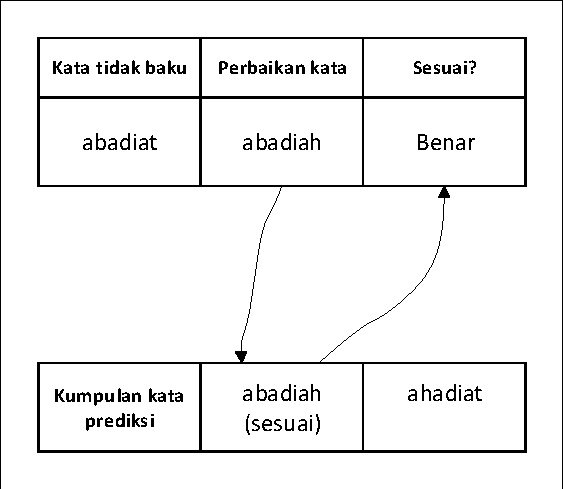
\includegraphics[width=0.6\textwidth, trim=2 2 2 2, clip]{resources/4/skenario1_eg.pdf}
	\caption{Contoh penilaian untuk pengujian skenario pertama}
	\label{fig:skenario1_eg}
\end{figure}

\subsection{Skenario Kedua: Melihat Seluruh Isi Kumpulan Kata}

Skenario kedua adalah penilaian dilakukan dengan melihat apakah terdapat perbaikan kata di dalam kumpulan kata prediksi. Contoh untuk skenario kedua dapat dilihat pada Gambar \ref{fig:skenario2_eg}. Seluruh kata dalam kumpulan kata prediksi diperiksa untuk menemukan salah satu kata yang sesuai dengan perbaikan kata. Jika ditemukan, maka kumpulan kata prediksi tersebut dianggap sesuai.
\begin{figure}[ht]
	\centering
	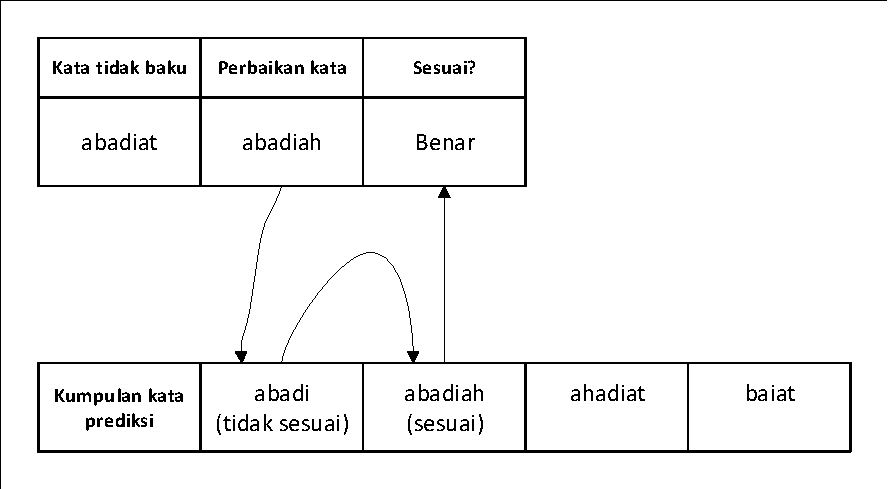
\includegraphics[width=0.8\textwidth, trim=2 2 2 2, clip]{resources/4/skenario2_eg.pdf}
	\caption{Contoh penilaian untuk pengujian skenario pertama}
	\label{fig:skenario2_eg}
\end{figure}

\section{Hasil Pengujian}

\subsection{Hasil Pengujian Skenario Pertama}

Hasil pengujian untuk skenario pengujian ditunjukkan pada Tabel \ref{tbl:result_1}. Hasil pengujian menunjukkan bahwa metode normalisasi yang diusulkan mengungguli kedua metode normalisasi yang lain dengan selisih akurasi dengan metode \parencite{saragih2017normalisasi} sebesar 6,35 persen. Metode normalisasi dengan Jaro-Winkler menempati peringkat terakhir dengan selisih akurasi dengan metode normalisasi \parencite{saragih2017normalisasi} sebesar 0,83 persen.
\begin{table}[ht]
    \captionsetup{justification=justified,singlelinecheck=false}
    \caption{Hasil akurasi untuk pengujian ketiga metode normalisasi dalam skenario pertama}
    \label{tbl:result_1}
    \centering
    \begin{tabularx}{\textwidth}{|X|c|c|c|}
        \hline
        \multicolumn{1}{|Y|}{\textbf{Metode}} & \textbf{Jumlah kata benar} & \textbf{Akurasi} \\ \hline
        Metode Normalisasi \parencite{saragih2017normalisasi} & 622 & 25,93\% \\ \hline
        Metode Normalisasi dengan Jaro-Winkler & 602 & 25,10\% \\ \hline
        Metode Normalisasi dengan Levenshtein & 774 & 32,28\% \\ \hline
    \end{tabularx}
\end{table}

Hasil metode normalisasi Jaro-Winkler yang berada di posisi terakhir disebabkan oleh teknik Jaro-Winkler dalam menentukan kemiripan antara kedua kata. Jaro-Winkler menganggap bahwa kedua kata dikatakan mirip jika terdapat karakter yang sesuai dengan jumlah yang banyak serta tidak ada transposisi dengan karakter yang sesuai tersebut. Maka, Jaro-Winkler akan menganggap kata dengan penambahan satu karakter memiliki kemiripan yang lebih tinggi dibandingkan kata dengan penggantian satu karakter saja, mengakibatkan kata yang mengalami penggantian karakter tergusur dari pencarian kata baku. Sebagai contoh, kata "\textit{asem}" memiliki kemiripan yang lebih tinggi dengan "rasem" dibandingkan dengan "asam", dengan nilai kemiripan masing-masing adalah 93,33 persen dan 86,67 persen.

Meskipun begitu, hasil akurasi pengujian untuk ketiga metode masih menunjukkan angka di bawah 50 persen. Hal tersebut disebabkan oleh perbaikan kata uji bukan merupakan kata yang berada dalam urutan pertama kumpulan kata prediksi. Hal tersebut berarti perbaikan kata uji bukan merupakan kata yang sering digunakan dalam korpus Kompas. Sebagai contoh, perbaikan kata "\textit{asem}" seharusnya adalah "asam", namun dalam metode normalisasi Levenshtein, kata "\textit{asem}" diidentifikasi sebagai "aset" yang mana "aset" adalah kata yang berada pada urutan pertama dalam kumpulan kata prediksi. Setelah melihat isi kumpulan kata prediksi, ternyata kata "asam" terdapat dalam kumpulan kata tersebut.

Untuk melihat adanya kata perbaikan yang masuk ke dalam kumpulan kata dengan jarak perubahan minimum, diperlukan skenario baru, yaitu dengan modifikasi algoritme penilaian pada ketiga metode normalisasi (skenario kedua). Gambar \ref{fig:skenario_side_to_side} menunjukkan perbedaan antara skenario pertama dengan skenario kedua. Jika skenario pertama hanya memeriksa urutan pertama dari kumpulan kata prediksi, skenario kedua memeriksa seluruh kumpulan kata prediksi hingga ditemukan kata yang sesuai dengan perbaikan kata.
\begin{figure}[ht]
	\centering
	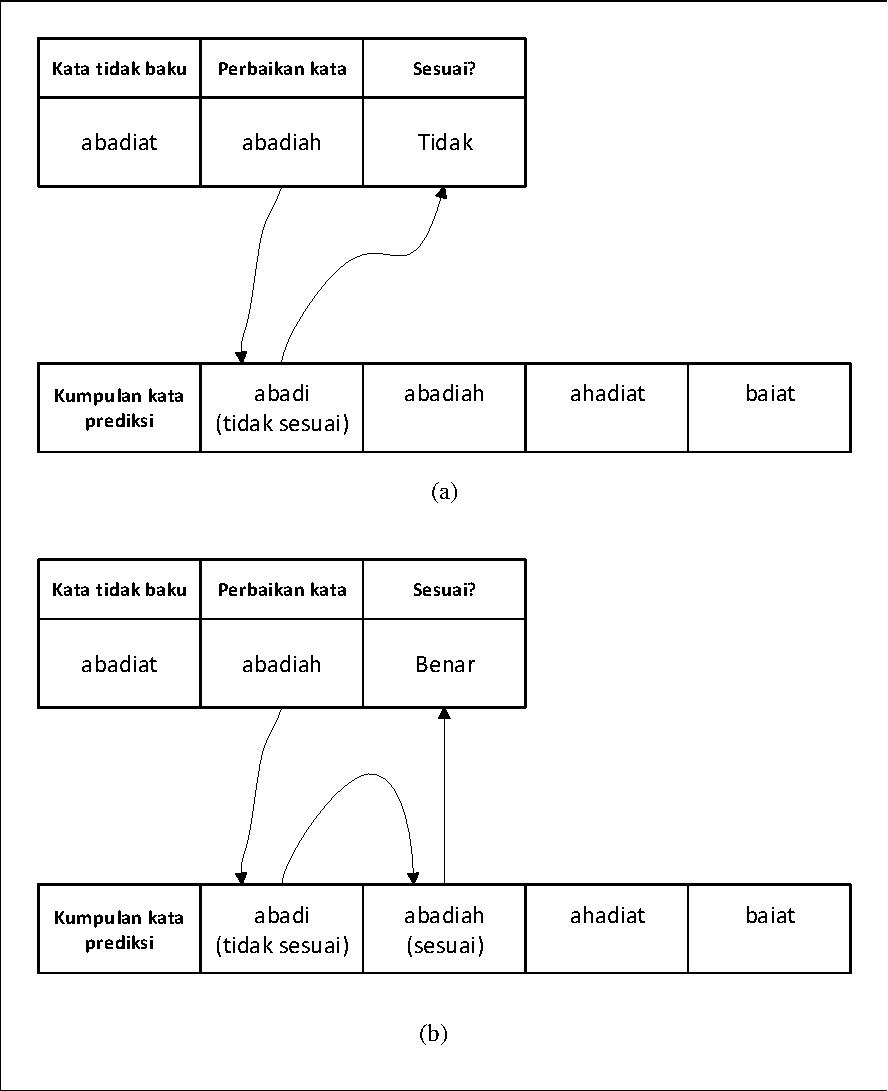
\includegraphics[width=0.5\textwidth, trim=2 2 2 2, clip]{resources/4/skenario_side_to_side.pdf}
	\caption{Perbedaan antara (a) skenario pertama, dan (b) skenario kedua}
	\label{fig:skenario_side_to_side}
\end{figure}

\subsection{Hasil Pengujian Skenario Kedua}

Hasil pengujian untuk skenario kedua disajikan pada Tabel \ref{tbl:result_2}, dan hasil untuk kedua pengujian dapat dilihat pada Gambar \ref{fig:ss_pengujian} Hasil pengujian tersebut menunjukkan peningkatan yang signifikan untuk selisih antara metode normalisasi Levenshtein dengan kedua metode normalisasi yang lain. Hasil akurasi untuk metode normalisasi Levenshtein masih mengungguli metode normalisasi \parencite{saragih2017normalisasi} dengan selisih sebesar 18,89 persen. Metode normalisasi dengan Jaro-Winkler masih tetap berada di posisi terakhir dengan selisih akurasi 21,6 persen dari metode normalisasi \parencite{saragih2017normalisasi}.
\begin{table}[ht]
    \captionsetup{justification=justified,singlelinecheck=false}
    \caption{Hasil akurasi untuk pengujian ketiga metode normalisasi dalam skenario kedua}
    \label{tbl:result_2}
    \centering
    \begin{tabularx}{\textwidth}{|X|c|c|c|}
        \hline
        \multicolumn{1}{|Y|}{\textbf{Metode}} & \textbf{Jumlah kata benar} & \textbf{Akurasi} \\ \hline
        Metode Normalisasi \parencite{saragih2017normalisasi} & 1233 & 51,42\% \\ \hline
        Metode Normalisasi dengan Jaro-Winkler & 715 & 29,82\% \\ \hline
        Metode Normalisasi dengan Levenshtein & 1686 & 70,31\% \\ \hline
    \end{tabularx}
\end{table}
\begin{figure}[ht]
	\centering
	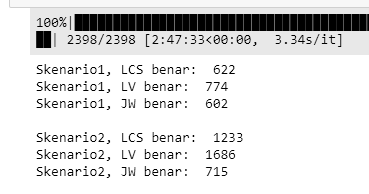
\includegraphics[width=0.7\textwidth, trim=2 2 2 2, clip]{resources/4/ss_pengujian.png}
	\caption{Seluruh hasil pengujian ketiga metode dengan menggunakan Jupyter Notebook}
	\label{fig:ss_pengujian}
\end{figure}

Hasil akurasi metode normalisasi dengan Jaro-Winkler yang masih di bawah 50 persen masih disebabkan oleh satuan penilaian kemiripan yang digunakan oleh Jaro-Winkler. Satuan penilaian yang digunakan adalah bilangan desimal, yang mana bilangan tersebut lebih sensitif terhadap perubahan dibandingkan dengan bilangan bulat. Hal tersebut mengakibatkan kumpulan kata dengan kemiripan tertinggi sementara tergusur dengan mudah oleh kata baru dengan kemiripan yang lebih tinggi, meskipun dengan selisih yang sangat kecil seperti 0.0001.

Meskipun hasil akurasi bertambah dibandingkan sebelumnya, persentase akurasi belum menyentuh angka 100 persen. Hal tersebut dapat disebabkan oleh jarak perubahan antara kata tidak baku dan perbaikan kata uji tidak termasuk dalam kumpulan kata dengan jarak perubahan minimum.Beberapa kata perbaikan dalam data uji memiliki jarak yag lebih besar dari jarak minimum yang ditemukan antara kata dalam data uji dengan beberapa kata dalam kamus kata baku. Sebagai contoh, kata "\textit{telepa}" merupakan kata tidak baku dari kata "telap" dan jarak perubahan antara kedua kata adalah 3 dengan jarak LCS dan 2 dengan jarak Levenshtein. Namun, ketiga metode normalisasi dapat menemukan kumpulan kata prediksi yang memiliki jarak perubahan yang lebih kecil dibandingkan jarak perubahan antara "\textit{telepa}" dan "telap" sehingga kata "telap" tidak dapat ditemukan.

Hasil pengujian tersebut menunjukkan bahwa masalah yang terjadi jika perbaikan kata uji telah diselesaikan, jika algoritme dalam metode normalisasi dapat melhat seluruh kata yang terkandung pada kumpulan kata prediksi. Namun, algoritme tersebut hanya dapat melihat kumpulan kata. Algoritme tidak dapat menentukan kata yang tepat digunakan, jika algoritme ingin diterapkan dalam sistem \textit{voice assistant}. Untuk penerapan dalam sistem \textit{voice assistant}, metode normalisasi juga harus dapat menentukan kata dalam kumpulan kata prediksi yang tepat digunakan.

\section{Kesimpulan Pengujian}

Pengujian yang telah dilakukan menghasilkan kesimpulan, bahwa metode normalisasi dengan jarak Levenshtein lebih cocok digunakan untuk digunakan sebagai normalisasi kata tidak baku yang tidak disingkat dibandingkan dengan metode normalisasi dengan jarak Jaro-Winkler. Hal tersebut ditunjukkan dengan unggulnya metode normalisasi dengan Levenshtein dalam semua skenario pengujian, sedangkan metode normalisasi dengan Jaro-Winkler tidak mampu mengungguli metode normalisasi \parencite{saragih2017normalisasi}.
    \chapter{Penutup}

\section{Kesimpulan}

Pengerjaan Tugas Akhir menunjukkan bahwa terdapat cara yang digunakan untuk mengatasi kata yang tidak tersedia pada kosakata sebuah bahasa. Cara yang digunakan adalah dengan menerapkan kategori "kata tidak diketahui" dan jarak Levenshtein untuk mencari kata yang mirip dengan yang ada di dalam kosakata. Diperlukan keputusan untuk menentukan seberapa jauh perbandingan sebuah kata dengan kata dalam kosakata sehingga diputuskan bahwa kata tersebut termasuk ke dalam "kata tidak diketahui".

\section{Saran}

Fungsi kosakata telah berjalan dengan baik, namun masih diperlukan perbaikan agar fungsi dapat menjadi lebih baik. Fungsi kosakata hanya dapat mencari kata yang mirip secara huruf-huruf yang dimiliki. Perlu dikembangkan lebih lanjut untuk fungsi kosakata sehingga fungsi kosakata diharapkan dapat mengetahui kata yang mirip secara makna.
    %----------------------------------------------------------------%

    % Daftar pustaka
    \clearpage
    \pagenumbering{roman}
    \setcounter{page}{\thesavepage}
    \addcontentsline{toc}{chapter}{Daftar Pustaka}
    \printbibliography[title=Daftar Pustaka]

    % Index
    \clearpage
    \appendix
    \addtocontents{toc}{\protect\renewcommand{\protect\cftchappresnum}{Lampiran }}
    \addtocontents{toc}{\protect\renewcommand{\protect\cftchapnumwidth}{6em}}
    \renewcommand{\chaptername}{Lampiran}
    \pagenumbering{bychapter}
    	
    \chapter{\textit{Source Code} Python untuk Jarak Levenshtein}

\begin{lstlisting}
def lv_distance(str1, str2):
    str1 = " " + str1
    str2 = " " + str2
    
    len1 = len(str1)
    len2 = len(str2)
    
    matrix = [[0] * len2 for i in range(len1)]
    
    for i in range(1, len1):
        matrix[i][0] = i
    for j in range(1, len2):
        matrix[0][j] = j
        
    for j in range(1, len2):
        for i in range(1, len1):
            actv = 1
            if (str1[i] == str2[j]):
                actv = 0
            matrix[i][j] = min(matrix[i-1][j] + 1, matrix[i][j-1] + 1, matrix[i-1][j-1] + actv)
    
    return matrix[len1-1][len2-1]
\end{lstlisting}
    \chapter{\textit{Source Code} Python untuk Normalisasi Kata dengan Jarak Levenshtein}

\begin{lstlisting}
def findWord_lv(txt, kam):
    minVal = 30
    similarWords = [txt]
    
    for word, i in kam.items():
        val = lv_distance(txt, word)
        if (val < minVal):
            if (val == 0):
                return [word], val
            else:
                similarWords = [word]
                minVal = val
        elif (val == minVal):
            similarWords.append(word)
            
    return similarWords, minVal
\end{lstlisting}
    
\end{document}
